\documentclass{article}
\usepackage{url,times,geometry}
\usepackage[utf8]{inputenc}
\usepackage[utf8]{vietnam}
\usepackage{graphicx}
\usepackage{float}
\usepackage{array}
\usepackage{longtable}
\graphicspath{ {./images/} }
\title{Luận văn tốt nghiệp}
\begin{document}
\maketitle

\section{Cơ sở lí thuyết và nền tảng công nghệ}
\subsection{Công nghệ Java }
\subsubsection{Java là gì}
Java là một ngôn ngữ lập trình được sử dụng rộng rãi được phát triển bởi Sun Microsystems vào năm 1995. Java có tính bảo mật cao và là một ngôn ngữ lập trình hướng đối
tượng. Đồng thời, một chương trình biết bằng Java có thể chạy được trên nhiều nền tảng và thiết bị khác nhau, cho phép người lập trình sử dụng một chương trình cho nhiều
nền tảng.

\subsubsection{Ưu điểm của Java}
Đầu tiên, Java là một ngôn ngữ lập trình hướng đối tượng, nghĩa là Java sử dụng các đối tượng được định nghĩa đầy đủ và mối quan hệ giữa các đối tượng khác nhau để thực
hiện các tác vụ khác nhau. Ngoài ra, Java còn sở hữu mọi ưu điểm của ngôn ngữ hướng đối tượng (có thể dùng lại code và mở rộng,...)
Thứ hai, Java là một ngôn ngữ đa nền tảng, sử dụng Java bytecode và Java Virtual Machine (JVM). Không như những ngôn ngữ khác được biên dịch trực tiếp thành mã máy trên
một nền tảng cụ thể, code Java sẽ được biên dịch thành một định dạng trung gian (bytecode) và được thực thi bởi JVM. Ta có thể viết một chương trình Java trên máy Windows
và thực thi nó trên máy Linux hoặc Mac OS, chỉ cần hai máy này có cài đặt môi trường Java.
\subsubsection{Nhược điểm của Java}
Nhược điểm lớn nhất của Java là tốc độ của nó chậm hơn so với các ngôn ngữ khác (PHP, ASP.NET..). Ngoài ra, ngôn ngữ Java tương đối khó để học đối với những người mới bắt
đầu học lập trình.
\subsection{Spring Framework }
Spring là một framework được viết bằng Java, Spring cung cấp cho người dùng nền tảng để phát triển ứng dụng Java. Spring cho phép người dùng xây dựng các ứng dụng từ các
“đối tượng Java cổ điển (POJOs)”, sau đây là một số ưu điểm của Spring:
   \begin{itemize}
     \item là một framework tương đối nhẹ (lighweigth).
     \item Được sử dụng nhiều cho các ứng dụng web vì hỗ trợ rất tốt các tính năng như web serices hay json...
     \item Hỗ trợ quản lý transaction, JDBC operations, File uploading, Exception Handling....
   \end{itemize}
   
\section{Thiết kế}

\subsection{Thiết kế cơ sở dữ liệu}

\subsubsection{Mô hình thực thể quan hệ}
\begin{figure}[H]
\centering
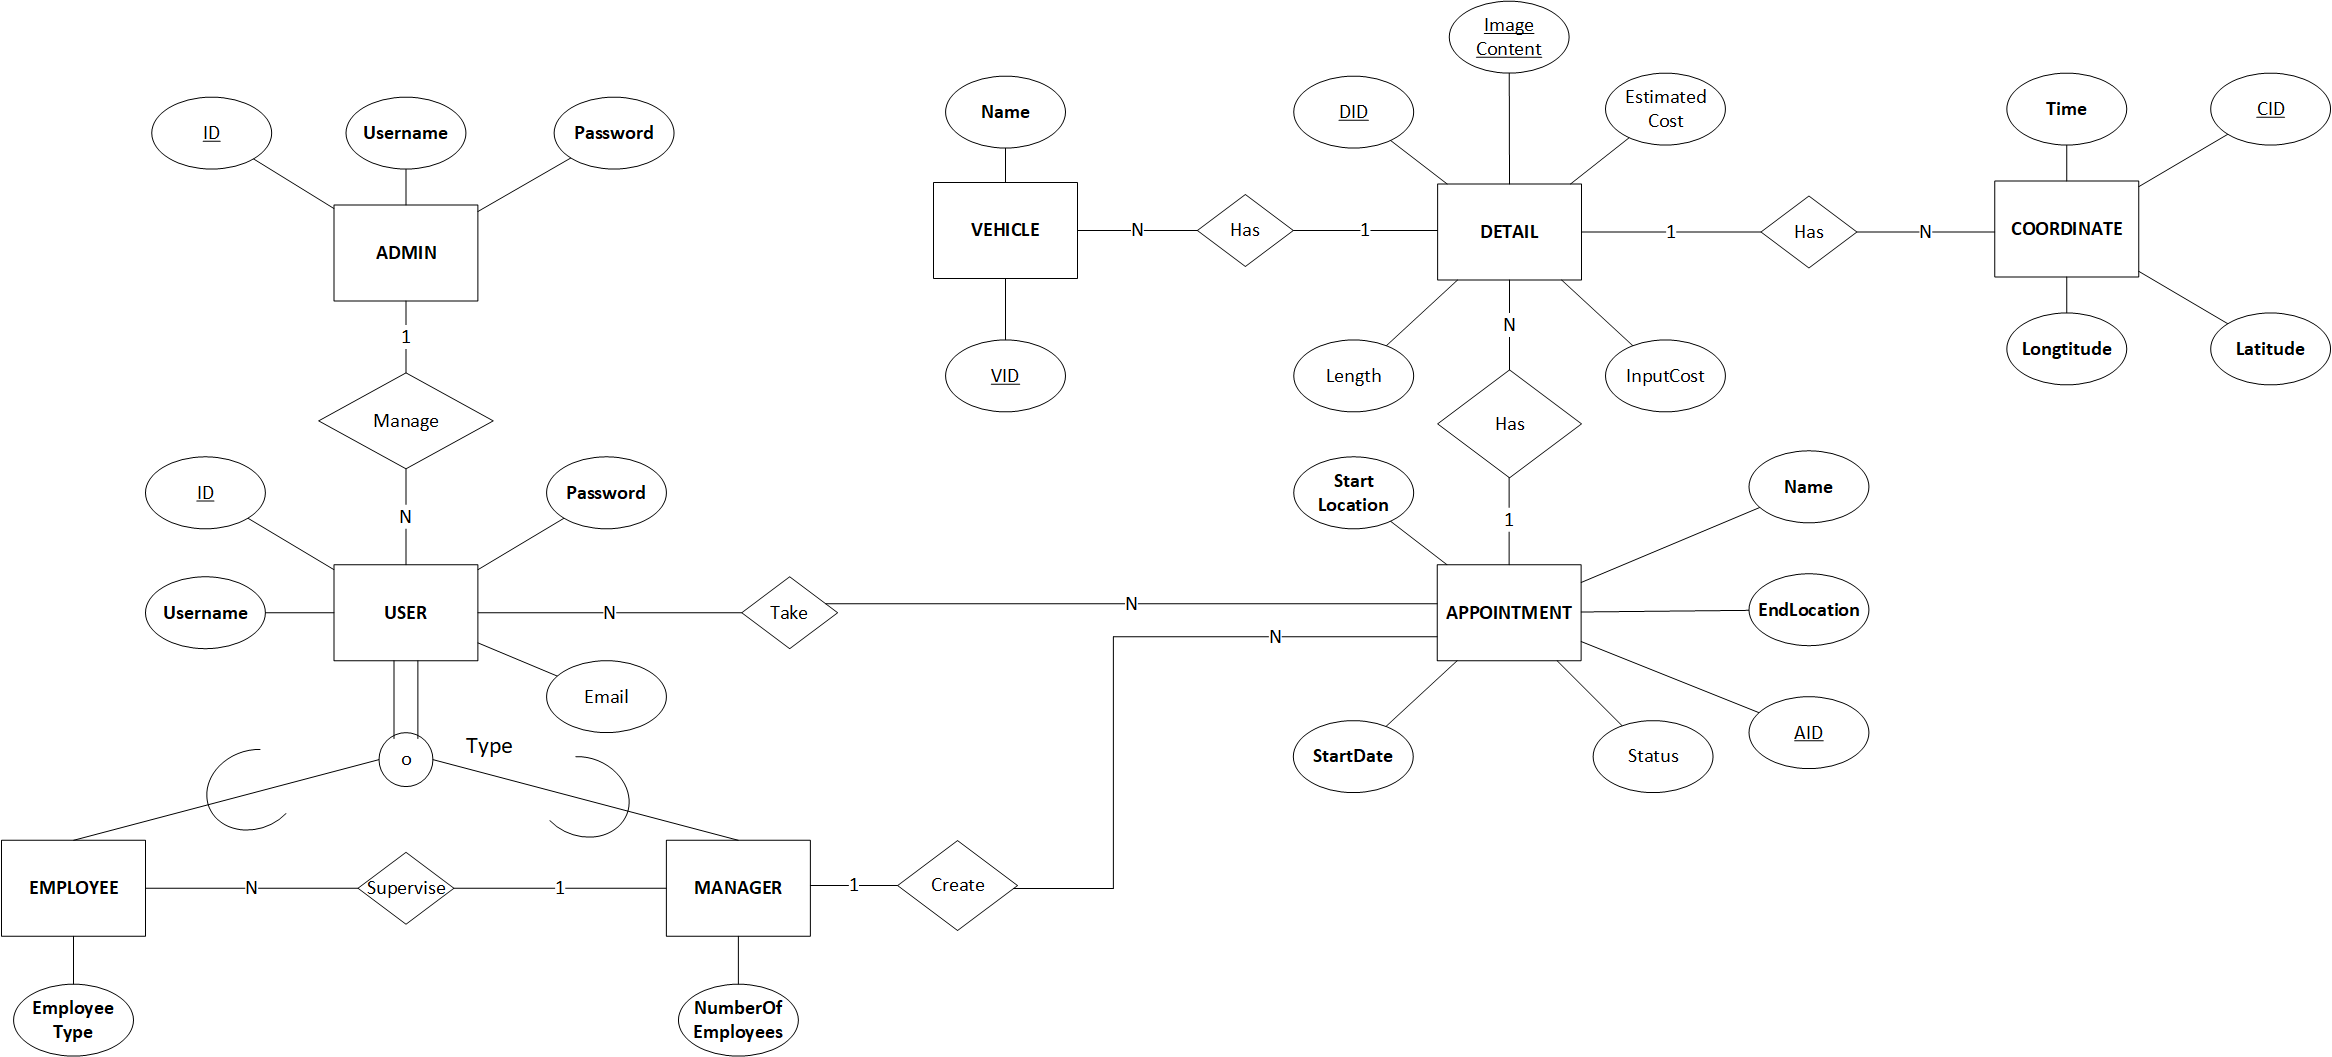
\includegraphics[angle=90, scale=0.32]{EERD_Diagram}
%height=12cm
\caption{Mô hình thực thể quan hệ}
\end{figure}

Các thực thể trong mô hình ERD trên: \newline
•	EMPLOYEE đại diện cho loại user nhân viên trong hệ thống.  \newline
•	MANAGER đại diện cho loại user manager trong hệ thống. \newline
•	ADMIN đại diện cho người quản trị trong hệ thống. \newline 
•	APPOINTMENT đại diện cho những cuộc hẹn với khách hàng hiện tại đã được tạo.\newline
•	DETAIL đại diện cho quảng đường mà người dùng đi được đối với một loại phương tiện. \newline
•	VEHICLE đại diện cho loại phương tiện mà người dùng sẽ lựa chọn để đi.\newline
•	COORDINATES đại diện cho tọa độ của người dùng trên bản đồ google maps. \newline

\subsubsection{Ánh xạ mô hình thực thể quan hệ}

\begin{figure}[H]
\centering
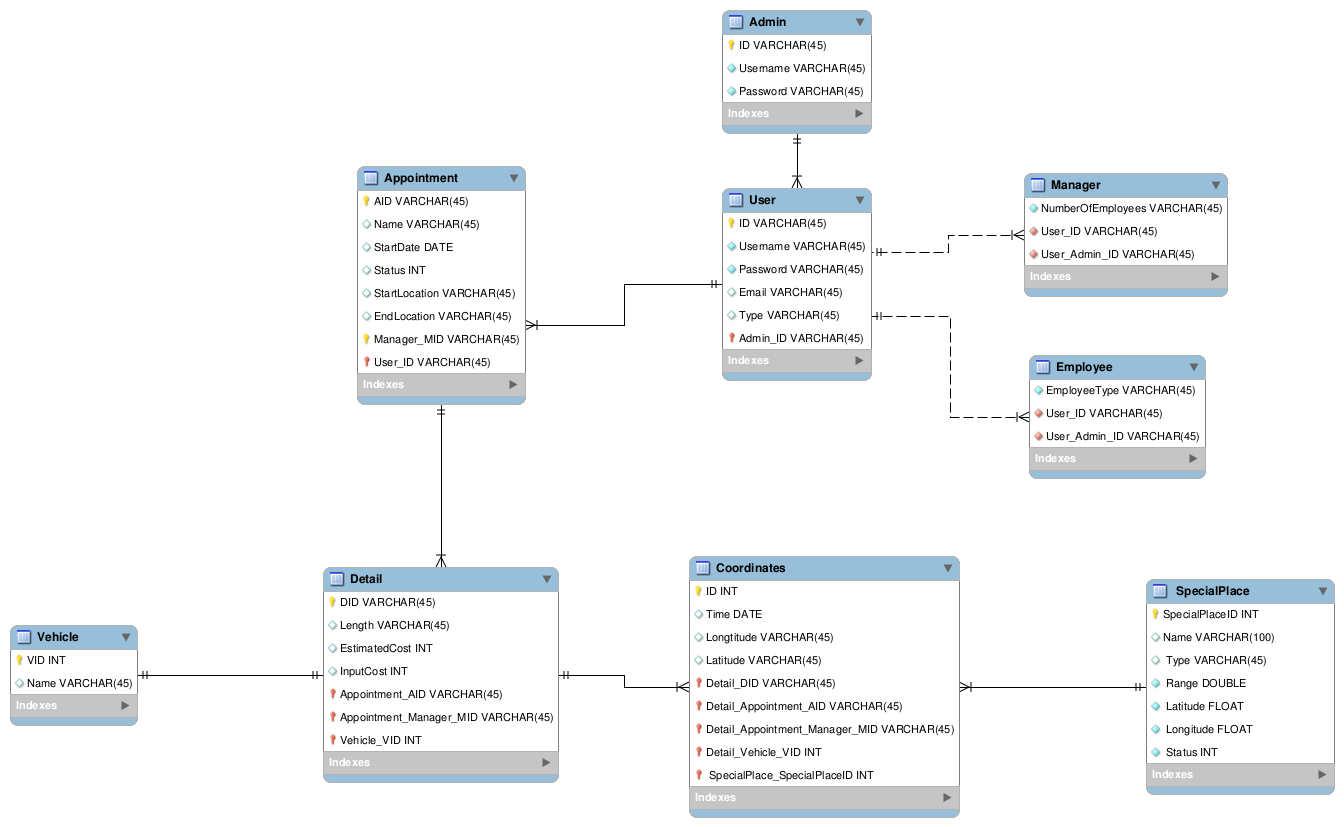
\includegraphics[scale=0.45, angle=90]{Database_Diagram}
\caption{Ánh xạ mô hình thực thể quan hệ}
\end{figure}

\subsection{Thiết kế giao diện}

\subsection{Thiết kế Activity Diagram biểu diễn cho phía server}
\begin{figure}[H]
\centering
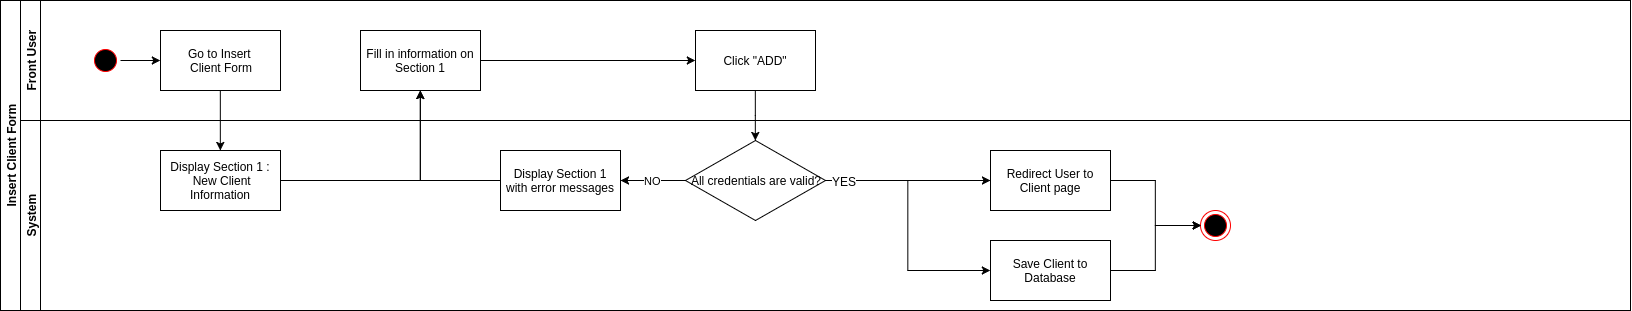
\includegraphics[scale=0.4]{themkhachhang}
\caption{Activity cho chức năng thêm khách hàng}
\end{figure}

\begin{figure}[H]
\centering
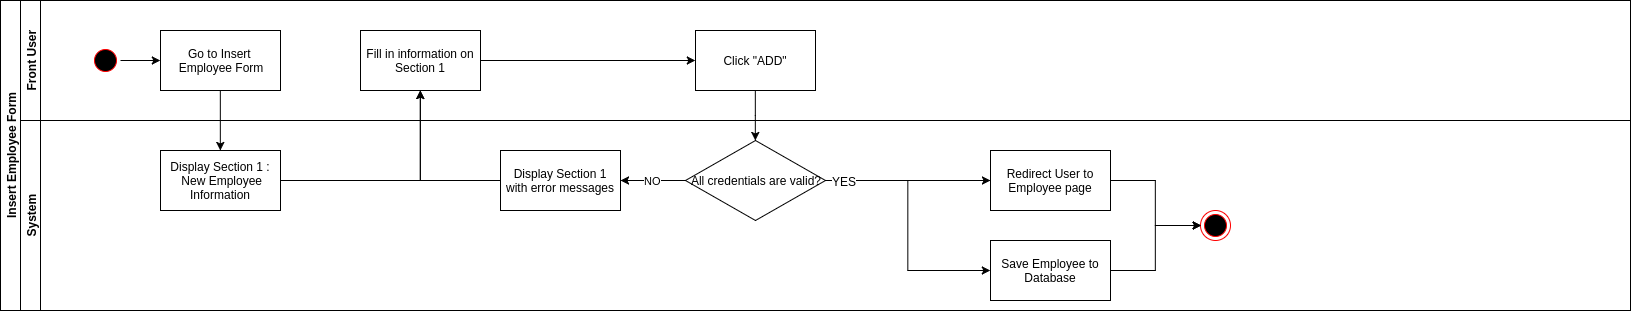
\includegraphics[scale=0.4]{themnhanvien}
\caption{Activity diagram cho chức năng thêm nhân viên}
\end{figure}

\begin{figure}[H]
\centering
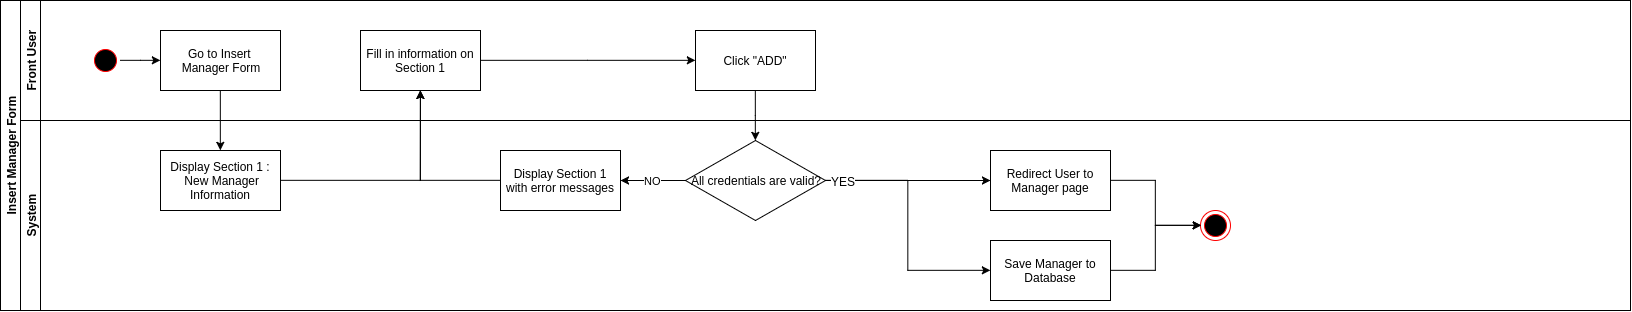
\includegraphics[scale=0.4]{themquanli}
\caption{Activity diagram cho chức năng thêm người quản lý}
\end{figure}

\begin{figure}[H]
\centering
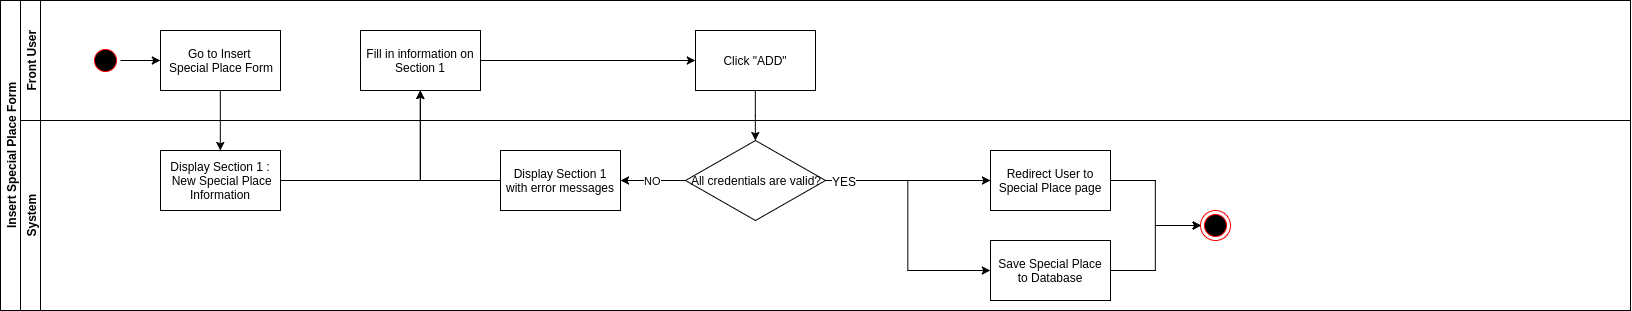
\includegraphics[scale=0.4]{themvitridacbiet}
\caption{Activity diagram cho chức năng thêm vị trí đặc biệt}
\end{figure}

\begin{figure}[H]
\centering
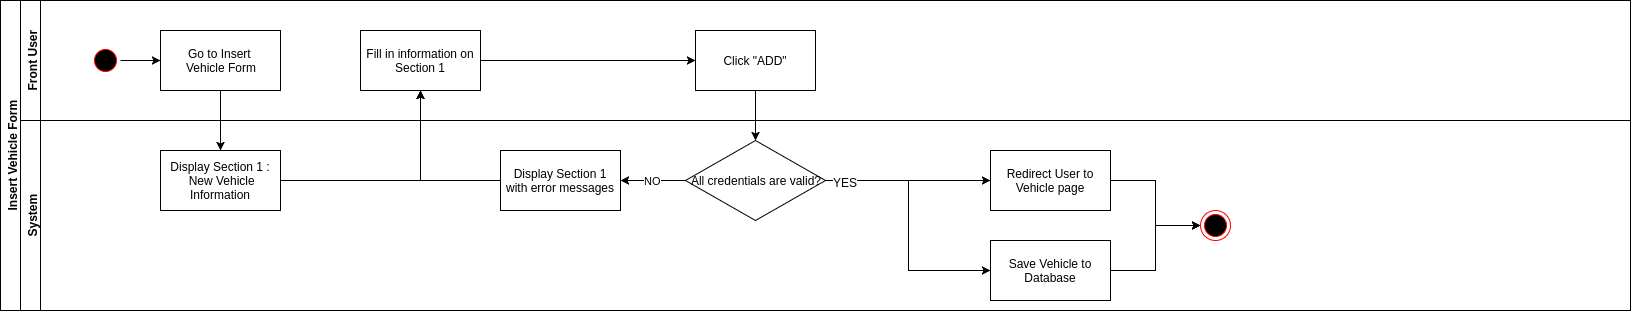
\includegraphics[scale=0.4]{themphuongtien}
\caption{Activity diagram cho chức năng thêm phương tiện}
\end{figure}

\begin{figure}[H]
\centering
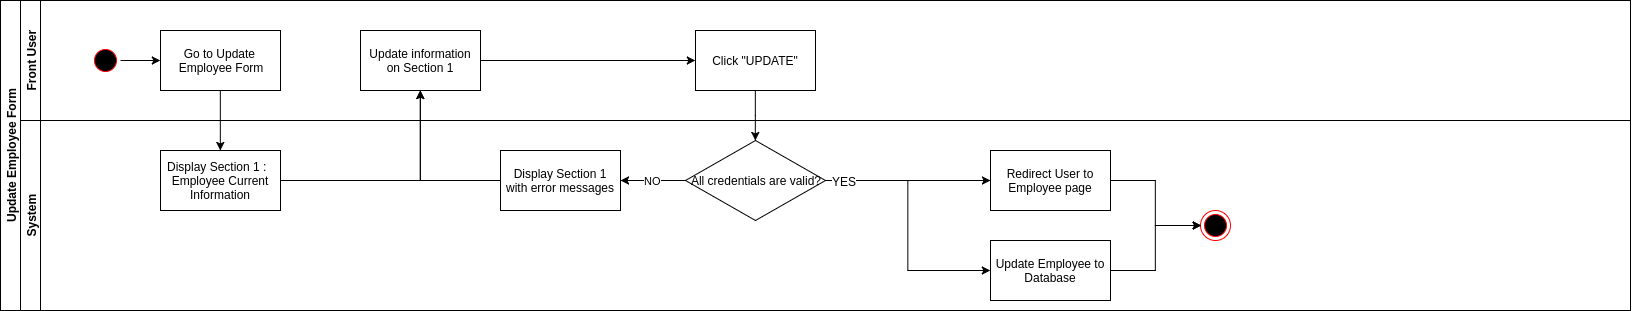
\includegraphics[scale=0.4]{chinhsuanhanvien}
\caption{Activity cho chức năng chỉnh sửa thông tin nhân viên}
\end{figure}

\begin{figure}[H]
\centering
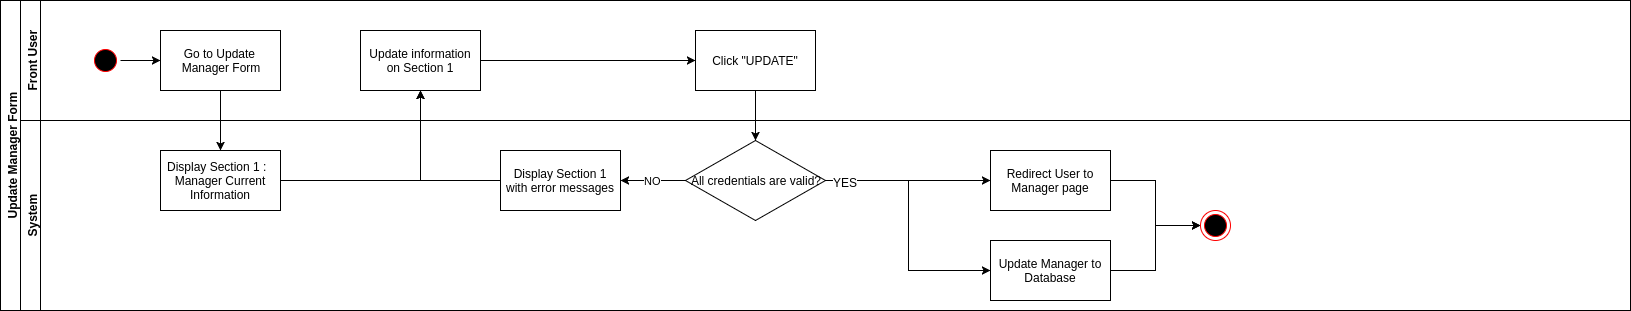
\includegraphics[scale=0.4]{chinhsuaquanli}
\caption{Activity cho chức năng chỉnh sửa thông tin manager}
\end{figure}

\begin{figure}[H]
\centering
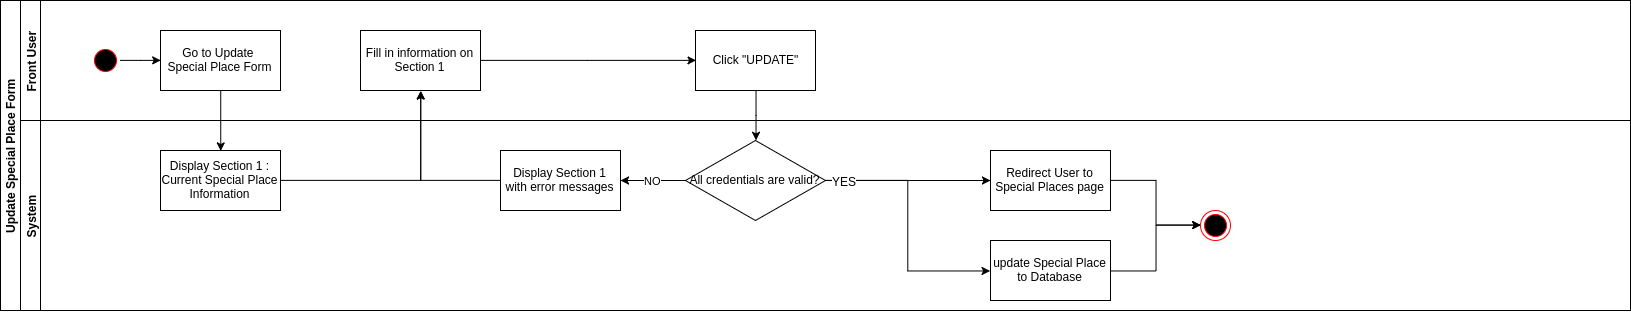
\includegraphics[scale=0.4]{chinhsuavitridacbiet}
\caption{Activity cho chức năng chỉnh sửa vị trí đặc biệt}
\end{figure}

\subsection{Danh sách các hàm được sử dụng}

\begin{longtable}{ | p{.20\textwidth} |p{.30\textwidth} | p{.50\textwidth}  | } 
\hline
\textbf{Tên hàm}& \textbf{Chức năng}& \textbf{Thông số đầu vào} \\ 
\hline

\hline
Create Appointment & 
Tạo một công tác và lưu vào trong cơ sở dữ liệu. &
Một JSON Object bao gôm các trường:
\begin{itemize}
  \item “destination” : đích đến của công tác(Chuỗi).
  \item “startdate” : ngày bắt đầu dự kiến của công tác(Chuỗi  có dạng HH:mm dd-MM-yyyy).
  \item “users” : danh sách mã số những người tham gia công tác(Chuỗi có dạng 1,2,3,4).
  \item “clientid” : mã số của khách hàng đã được lưu trong cơ sở dữ liệu(Số  nguyên). 
\end{itemize}
  \\ 
\hline
Get Active Appointments & 
Lấy danh sách các công tác chưa kết thúc trong cơ sở dữ liệu. &
không có tham số nào. \\

\hline
Get Completed Appointments & 
Lấy danh sách các công tác đã kết thúc trong cơ sở dữ liệu. &
không có tham số nào. \\ 

\hline
Update Appointment & 
Cập nhật thông tin một công tác đã tồn tại trong cơ sở dữ liệu (chỉ dùng cho người quản lý). &
Một JSON Object bao gôm các trường: 
\begin{itemize}
  \item “\verb|destination|” : đích đến của công tác (Chuỗi). 
  \item “\verb|start_date|” : ngày bắt đầu dự kiến của công tác (Chuỗi  có dạng HH:mm dd-MM-yyyy).
  \item “\verb|users|” : danh sách mã số những người tham gia công tác(Chuỗi có dạng 1,2,3,4).
  \item “\verb|client_id|” : mã số của khách hàng đã được lưu trong cơ sở dữ liệu(Số  nguyên).
  \item “\verb|appointment_id|” : mã số của công tác ta muốn cập nhật (Số nguyên). 
\end{itemize}
\\ 

\hline
End Appointment  & 
Kết thúc một công tác và cập nhật vào cơ sở dữ liệu. &
Một JSON Object bao gôm các trường: 
\begin{itemize}
  \item “\verb|id|” : mã số của công tác (Số nguyên).  
  \item “\verb|end_date|” : thời gian kết thúc của công tác (Chuỗi có dạng HH:mm dd-MM-yyyy).
\end{itemize}
\\ 

\hline
Create Client & 
Tạo một khách hàng và lưu vào trong cơ sở dữ liệu. &
Một JSON Object bao gôm các trường: 
\begin{itemize}
  \item “\verb|name|” : tên của khách hàng (Chuỗi).  
  \item “\verb|phone_number|” :số điện thoại của khách hàng (Chuỗi số bao gôm 10-11 số nhất và chỉ được thêm khoảng trắng). 
  \item “\verb|address|” :  địa chỉ của khách hàng (Chuỗi).
  \item “\verb|email|” : email của khách hàng (Chuỗi tuân theo đúng định dạng email).
\end{itemize}
\\ 

\hline
Get Clients & 
Lấy danh sách các khách hàng đã lưu trong cơ sở dữ liệu. &
không có thông số nào.
\\ 

\hline
Get Client Info & 
Lấy thông tin chi tiết của một khách hàng . &
Một JSON Object chứa một trường duy nhất là mã số của khách hàng (Số nguyên).
\\ 

\hline
Add Coordinate & 
Thêm một (hoặc nhiều) tọa độ vị trí cho một lịch trình. &
Một JSON Object bao gôm các trường: 
\begin{itemize}
  \item “\verb|detail_id|” : mã số của lịch trình.  
\item “\verb|coordinates|” :mảng các tọa độ (JSON Array) có cấu trúc của một phần tử bao gồm ba trường : “latitude” (vĩ độ - Số thực), “longitude”(kinh độ - số thực) và
“time”(thời gian - chuỗi có dạng HH:mm:ss dd-MM-yyyy).
\end{itemize}
\\ 

\hline
Create Detail & 
Tạo một lịch trình và lưu vào trong cơ sở dữ liệu, đồng thời ta cũng bắt đầu luôn lịch trình này. &
Một JSON Object bao gôm các trường: 
\begin{itemize}
  \item “\verb|vehicle_id|” : : mã số của phương tiện (Số nguyên).  
  \item “\verb|start_time|” : thời gian bắt đầu của lịch trình (Chuỗi  có dạng HH:mm:ss dd-MM-yyyy).
  \item “\verb|start_location|”: thời gian bắt đầu của lịch trình (Chuỗi  có dạng HH:mm:ss dd-MM-yyyy).
  \item “\verb|appointment_id|”: mã số của công tác đã được lưu trong cơ sở dữ liệu (Số  nguyên). 
\end{itemize}
\\ 


\hline
End Detail  & 
Kết thúc một lịch trình. &
Một JSON Object bao gôm các trường: 
\begin{itemize}
  \item “\verb|image_content|” : hình ảnh hóa đơn được người dùng chụp lại, đây là một chuỗi có nội dung là base 64 của file hình ảnh, có thể rỗng. 
  \item “\verb|description|” : ghi chú của lịch trình này (kẹt xe, bể bánh, thêm tiền...) (Chuỗi).
  \item “\verb|input_cost|”: số tiền phải trả để thực hiện lịch trình (Số thực).
\end{itemize}
\\ 

\hline
Get Employees & 
Lấy danh sách các nhân viên dưới quyền quản lý (chỉ dùng cho người quản lý).&
Một JSON Object bao một trường duy nhất là mã số của người dùng (Số nguyên).
\\ 

\hline
Get User Info  & 
Lấy thông tin chi tiết của một người dùng. &
Một JSON Object bao một trường duy nhất là mã số của người dùng (Số nguyên).
\\

\hline
Get Vehicles   & 
Lấy danh sách các phương tiện đi lại. &
không có tham số nào.
\\
 
\hline

\caption{Bảng các hàm chính được sử dụng của hệ thống}
\end{longtable}

\section{Hiện thực}
\subsection{Công nghệ sử dụng}
Để hiện thực đề tài này, chúng tôi sử dụng một số công nghệ và ứng dụng sau : 
\begin{longtable}{ | p{.20\textwidth} |p{.30\textwidth} | p{.50\textwidth}  | } 
\hline
\textbf{Công nghệ và ứng dụng}& \textbf{Phiên bản}& \textbf{Ghi chú} \\ 
\hline
\hline
Spring Framework &
4.0.6 &
Công nghệ chủ đạo của phía Server.
\\ 
\hline
Android  &
5.0 trở lên &
Công nghệ chủ đạo của phía Client.
\\ 
\hline
Java  &
8.0 &
Công nghệ chủ đạo của phía Client.
\\ 
\hline
Apache  &
2.2.11 &
Công nghệ chủ đạo của phía Client.
\\ 
\hline
PostgreSQL  &
10 &
Cơ sở dữ liệu của toàn bộ hệ thống.
\\ 

\hline

\caption{Bảng các công nghệ sử dụng}
\end{longtable}

\subsection{Phiên bản mẫu Client}

\subsection{Phiên bản mẫu Server}
Sau đây nhóm xin trình bày một số phiên bản mẫu (phần còn lại vui lòng xem lại ở phụ lục phần 4) :
\subsubsection{Trang chủ của hệ thống}
Trang chủ của hệ thống hiển thị giao diện mà hệ thống hiện ra cho người quản trị sau khi người quản trị đăng nhập thành công. Người quản trị sẽ dùng menu hiện ra ở phía
bên tay trái để đi đến các trang web khác.

\begin{figure}[H]
\centering
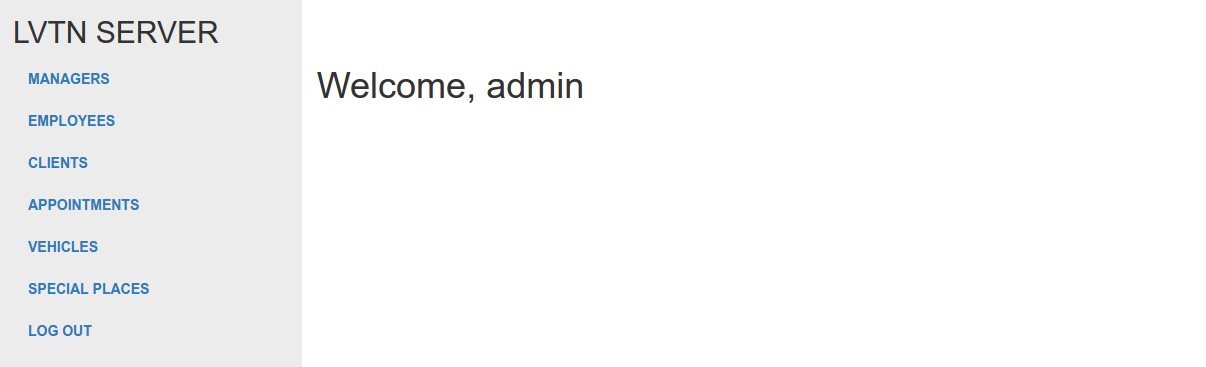
\includegraphics[scale=0.5]{admin_trangchu}
\caption{Màn hình trang chủ}
\end{figure}

\subsubsection{Trang thêm, cập nhật công thức dự đoán chi phi phương tiện}
Trang này dự cho phép người sử dụng thêm hoặc cập nhật lại một công thức dự đoán chi phí của một phương tiện dựa vào thời gian và quãng đường sử dụng phương tiện đó. Hiện
tại hệ thống hỗ trợ cho người dùng những phép toán cộng trừ nhân chia cơ bản.

\begin{figure}[H]
\centering
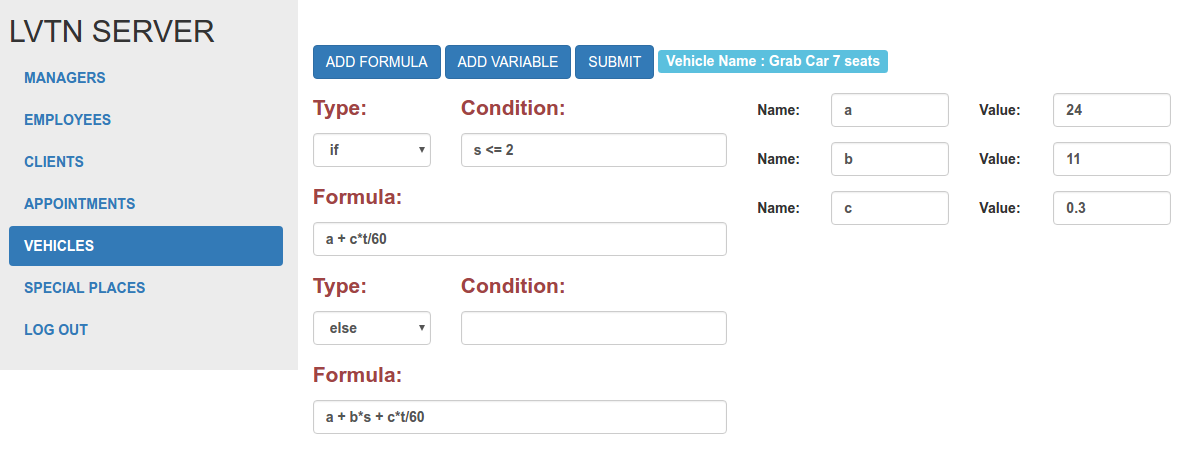
\includegraphics[scale=0.5]{admin_chiphi}
\caption{Màn hình cập nhật công thức dự đoán chi phí phương tiện}
\end{figure}


\subsubsection{Chức năng quản lý của người quản trị}
Hiện thực tất cả các chức năng quản lý của người quản trị bao gồm quản lý người dùng, quản lý khách hàng, quản lý phương tiện, quản lý danh sách các vị trí đặc biệt.
Những hình bên dưới là phiên bản quản lý người dùng với các chức năng xem, tìm kiếm, sắp xếp, thêm, chỉnh sửa, vô hiệu hóa và thống kê.

\begin{figure}[H]
\centering
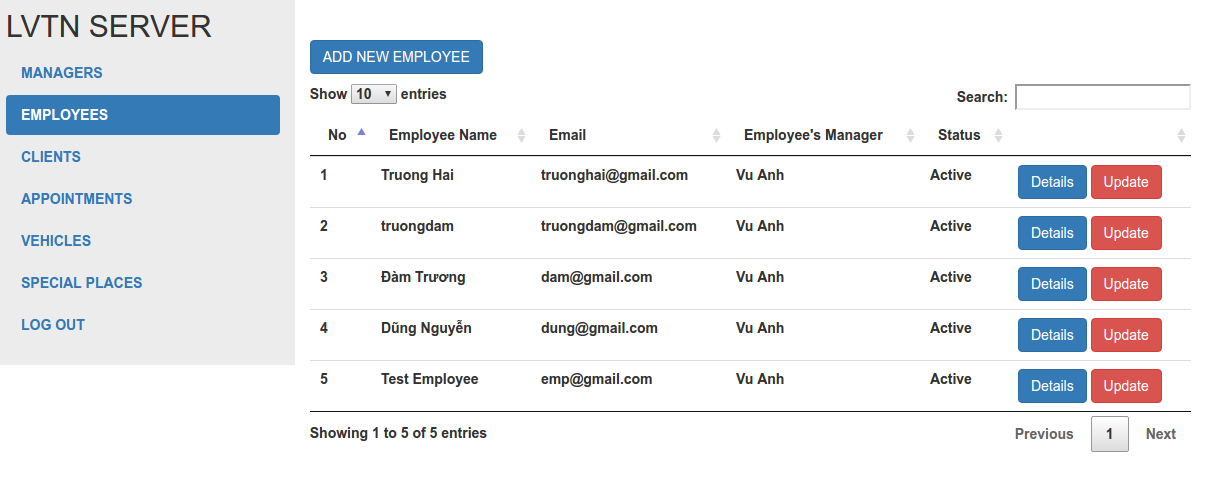
\includegraphics[scale=0.5]{admin_employee}
\caption{Màn hình quản lí nhân viên}
\end{figure}


\begin{figure}[H]
\centering
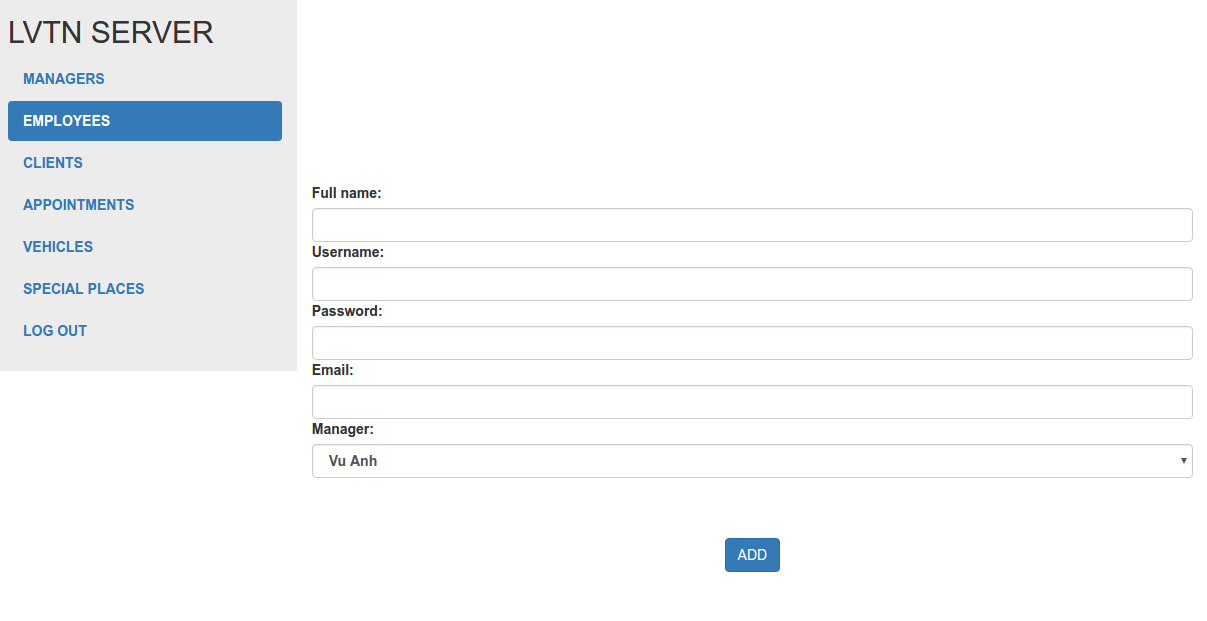
\includegraphics[scale=0.5]{admin_themnhanvien}
\caption{Màn hình quản lí thêm nhân viên}
\end{figure}

\begin{figure}[H]
\centering
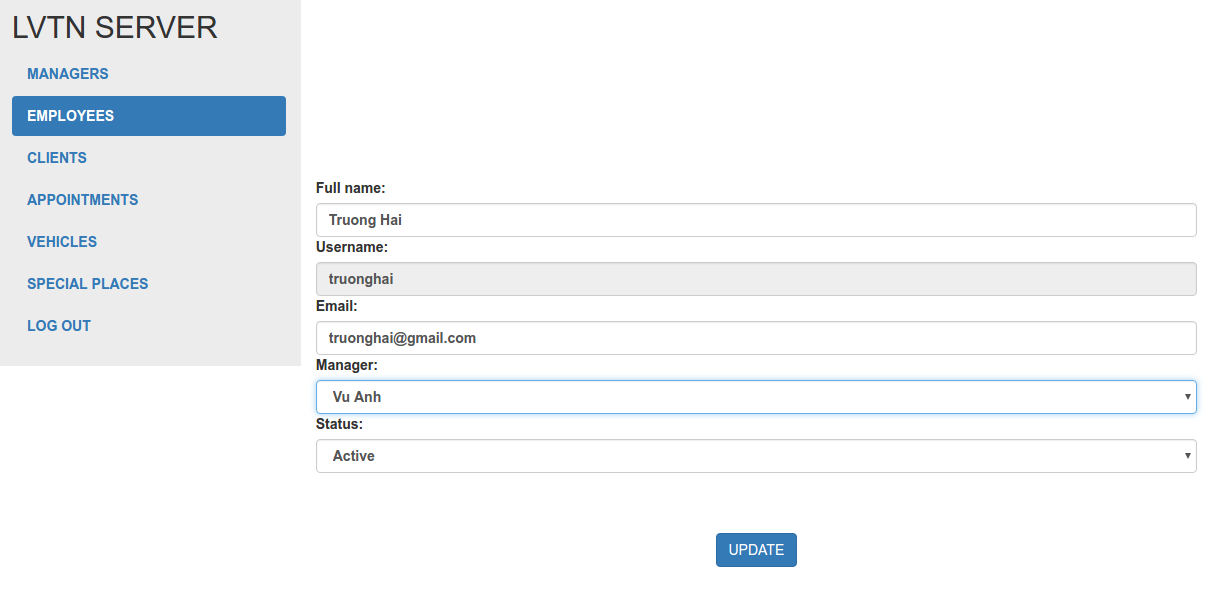
\includegraphics[scale=0.5]{admin_chinhsuanhanvien}
\caption{Màn hình quản lí chỉnh sửa thông tin nhân viên}
\end{figure}

\begin{figure}[H]
\centering
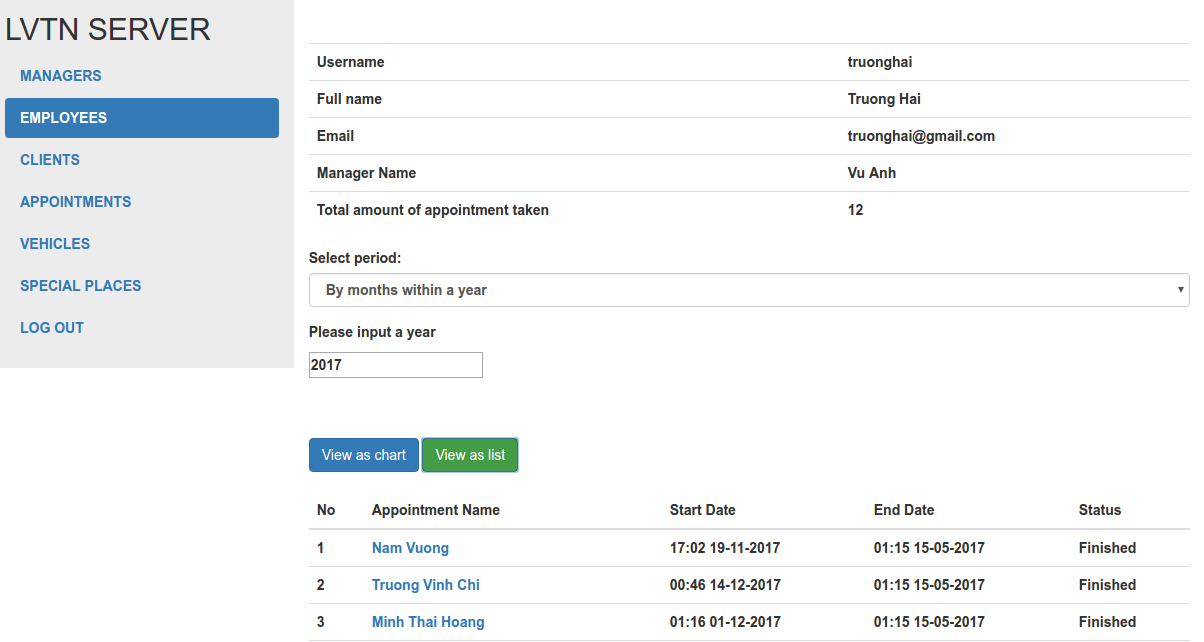
\includegraphics[scale=0.5]{admin_lichtrinh}
\caption{Màn hình quản lí các lịch trình của nhân viên}
\end{figure}

\begin{figure}[H]
\centering
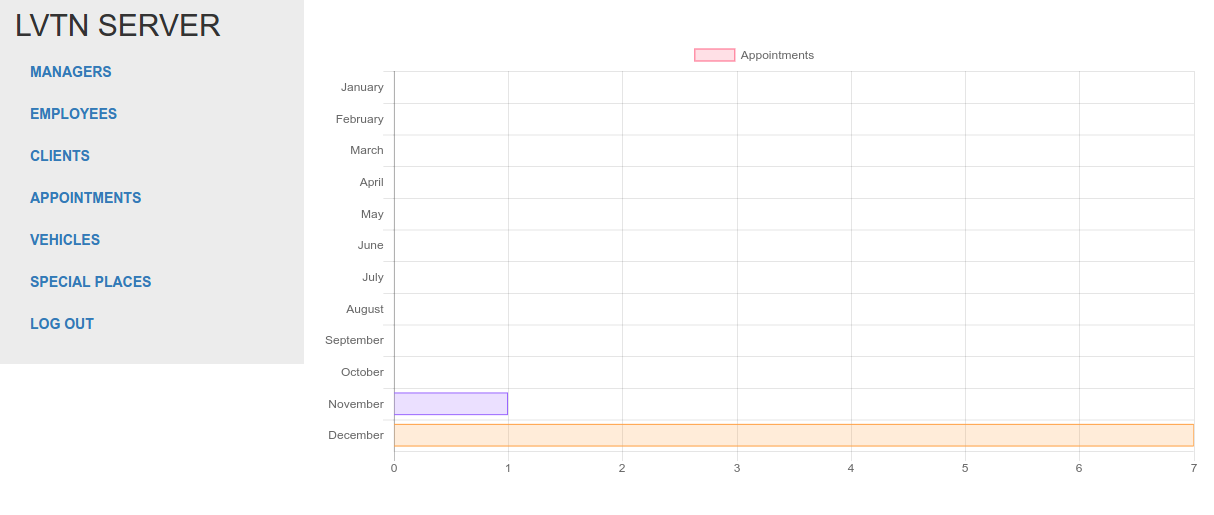
\includegraphics[scale=0.5]{admin_lichtrinhchart}
\caption{Màn hình thể hiện các lịch trình của nhân viên theo biểu đồ}
\end{figure}


\subsection{Thiết kế bản kiểm thử (những chức năng chính)}
Sau đây nhóm xin trình bày một số phiên bản mẫu (phần còn lại vui lòng xem lại ở phụ lục phần 3) : 
\subsubsection {Chức năng đăng nhập vào hệ thống}

\begin{longtable}{ | p{.15\textwidth} |p{.30\textwidth} | p{.35\textwidth}  | p{.10\textwidth}  | p{.10\textwidth}  | } 
\hline
\textbf{Testcase}& \textbf{Bước thực hiện}& \textbf{Kết quả đạt được} & \textbf{Đã kiểm tra}& \textbf{Đạt} \\ 
\hline
\hline
Đăng nhập vào hệ thống với hai trường username và password đều trống &
Các bước thực hiện: \newline
- Truy cập vào đường dẫn trang web. \newline
- Bỏ trống cả hai trường username và password. \newline
- Bấm vào nút “LOGIN”
&
Hệ thống sẽ trả về lỗi : \newline
- username cannot be empty and must be within 4 to 32 characters. \newline
- password cannot be empty and must be within 4 to 32 characters.
&
Đã kiểm tra &
Đạt \\

\hline
Đăng nhập vào hệ thống với một trong hai trường bị bỏ trống. &
Các bước thực hiện: \newline
- Truy cập vào đường dẫn trang web. \newline
- Bỏ trống một trong hai trường username hoặc password.  \newline
- Bấm vào nút “LOGIN”. 
&
Hệ thống sẽ trả về lỗi : \newline
- Nếu ta bỏ trống trường username : username cannot be empty and must be within 4 to 32 characters. \newline
- Nếu ta bỏ trống trường password : password cannot be empty and must be within 4 to 32 characters . \newline
&
Đã kiểm tra &
Đạt \\

\hline
Đăng nhập vào hệ thống với cả hai trường username và password có độ dài bé hơn 4 hoặc lớn hơn 32 ký tự &
Các bước thực hiện: \newline
- Truy cập vào đường dẫn trang web. \newline
- Nhập vào trường username và password giá trị “abc”.  \newline
- Bấm vào nút “LOGIN”.
&
Hệ thống sẽ trả về lỗi : \newline
- username cannot be empty and must be within 4 to 32 characters. \newline
- password cannot be empty and must be within 4 to 32 characters. \newline
&
Đã kiểm tra &
Đạt \\

\hline
Đăng nhập vào hệ thống với trường username có độ dài bé hơn 4 ký tự và lớn hơn 32 ký tự &
Các bước thực hiện: \newline
- Truy cập vào đường dẫn trang web.  \newline
- Nhập vào trường username giá trị “abcd” và password giá trị “abcdefgh”.  \newline
- Bấm vào nút “LOGIN”.
&
Hệ thống sẽ trả về lỗi : \newline
username cannot be empty and must be within 4 to 32 characters \newline
&
Đã kiểm tra &
Đạt \\


\hline
Đăng nhập vào hệ thống với trường password có độ dài bé hơn 4 ký tự và lớn hơn 32 ký tự &
Các bước thực hiện: \newline
- Truy cập vào đường dẫn trang web. \newline
- Nhập vào trường username giá trị “abcdefgh” và password giá trị “abd”. \newline
- Bấm vào nút “LOGIN”.
 &
Hệ thống sẽ trả về lỗi : \newline
- password cannot be empty and must be within 4 to 32 characters.
 &
Đã kiểm tra &
Đạt \\

\hline
Đăng nhập vào hệ thống với hai (hoặc một trong hai) trường username và password sai  &
Các bước thực hiện: \newline
- Truy cập vào đường dẫn trang web. \newline
- Nhập vào trường username giá trị “admin” và password giá trị “admin1”.  \newline
- Bấm vào nút “LOGIN”
&
Hệ thống sẽ trả về lỗi : Invalid username or password.
&
Đã kiểm tra &
Đạt \\

\hline
Đăng nhập vào hệ thống với cả hai trường username và password đã tồn tại trong database &
Các bước thực hiện: \newline
- Truy cập vào đường dẫn trang web. \newline
- Nhập vào trường username giá trị “admin” và password giá trị “admin”.  \newline
- Bấm vào nút “LOGIN”
&
Hệ thống sẽ đưa ta đến trang chủ. Đăng nhập thành công. &
Đã kiểm tra &
Đạt \\
\hline
\caption{Bảng kiểm thử đăng nhập vào hệ thống}
\end{longtable}

\subsubsection{Thao tác đối với trang Lịch trình (Appointments)}
\begin{longtable}{ | p{.15\textwidth} |p{.30\textwidth} | p{.35\textwidth}  | p{.10\textwidth}  | p{.10\textwidth}  | } 
\hline
\textbf{Testcase}& \textbf{Bước thực hiện}& \textbf{Kết quả đạt được} & \textbf{Đã kiểm tra}& \textbf{Đạt} \\ 
\hline
\hline
Kiểm tra chức năng cho phép người dùng chọn trạng thái của lịch trình &
Các bước thực hiện: \newline
- Chọn dropdown list nằm ở dưới nhãn : “Select the status of appointments:”. \newline
- Thay đổi giá trị của dropdown list này (giá trị mặc định đang là “View all”).
&
Hệ thống sẽ trả về danh sách các lịch trình có trạng thái (Status) tương ứng với giá trị dropdown list mà ta vừa đổi. &
Đã kiểm tra &
Đạt \\

\hline
Kiểm tra chức năng tìm kiếm của bảng dữ liệu &
Các bước thực hiện: \newline
- Chọn ô tìm kiếm trong bảng dữ liệu. \newline
- Nhập vào một giá trị nào đó. 
&
Dữ liệu trong bảng sẽ thay đổi, hệ thống sẽ chỉ hiện ra những lịch trình có liên quan đến từ khóa ta nhập vào. &
Đã kiểm tra &
Đạt \\

\hline
Kiểm tra chức năng tìm kiếm theo từng cột của bảng dữ liệu &
Các bước thực hiện:
Chọn một cột trong bảng dữ liệu. \newline
- Bấm vào tên của cột đó.  \newline
&
Dữ liệu trong bảng sẽ được sắp xếp lại theo giá trị của cột ta đã chọn theo chiều tăng dần hoặc giảm dần. &
Đã kiểm tra &
Đạt \\

\hline
Kiểm tra chức năng paging của bảng &
Các bước thực hiện: \newline
- Chọn dropdown list nằm ngang với nhãn “Show...entries:”.  \newline
- Giá trị mặc định là 10 hàng một trang, ta tiến hành đổi giá trị này. Nếu số trang của bảng dữ liệu lớn hơn một, ta tiến hành bầm các nút “Previous”,”Next” hoặc bấm vào số thứ tự của trang.
&
Hệ thống sẽ trả về dữ liệu tương ứng với những giá trị ta thay đổi. &
Đã kiểm tra &
Đạt \\


\hline
Kiểm tra thông tin chi tiết của một lịch trình &
Các bước thực hiện: \newline
-  Chọn một lịch trình trong bảng dữ liệu. \newline
-  Bấm vào nút “Details” tương ứng với lịch trình đó (nút này sẽ nàm cùng hàng với lịch trình). &
Hệ thống sẽ đưa ta đến trang thông tin chi tiết của lịch trình.&
Đã kiểm tra &
Đạt \\

\hline
\caption{Bảng kiểm thử thao tác trang Lịch trình}
\end{longtable}

%Managers 
\subsubsection{Thao tác đối với trang Người quản lý  (Managers)}
\begin{longtable}{ | p{.15\textwidth} |p{.30\textwidth} | p{.35\textwidth}  | p{.10\textwidth}  | p{.10\textwidth}  | } 
\hline
\textbf{Testcase}& \textbf{Bước thực hiện}& \textbf{Kết quả đạt được} & \textbf{Đã kiểm tra}& \textbf{Đạt} \\ 
\hline
\hline
Kiểm tra chức năng cho phép người dùng thêm người quản lý mới &
Các bước thực hiện: \newline
- Bấm vào nút “ADD NEW MANAGER.
&
Hệ thống sẽ đưa người dùng đến trang thêm người quản lý mới. &
Đã kiểm tra &
Đạt \\

\hline
Kiểm tra chức năng tìm kiếm của bảng dữ liệu. &
Các bước thực hiện: \newline
- Chọn ô tìm kiếm trong bảng dữ liệu. \newline
- Nhập vào một giá trị nào đó. 
&
Dữ liệu trong bảng sẽ thay đổi, hệ thống sẽ chỉ hiện ra những lịch trình có liên quan đến từ khóa ta nhập vào. &
Đã kiểm tra &
Đạt \\

\hline
Kiểm tra chức năng tìm kiếm theo từng cột của bảng dữ liệu. &
Các bước thực hiện: \newline
- Chọn một cột trong bảng dữ liệu.  \newline
- Bấm vào tên của cột đó. 
&
Dữ liệu trong bảng sẽ được sắp xếp lại theo giá trị của cột ta đã chọn theo chiều tăng dần hoặc giảm dần. &
Đã kiểm tra &
Đạt \\

\hline
Kiểm tra chức năng paging của bảng. &
Các bước thực hiện: \newline
- Chọn dropdown list nằm ngang với nhãn "Show...entries:".   \newline
- Giá trị mặc định là 10 hàng một trang, ta tiến hành đổi giá trị này. \newline
- Nếu số trang của bảng dữ liệu lớn hơn một, ta tiến hành bầm các nút “Previous”,”Next” hoặc bấm vào số thứ tự của trang.
&
Hệ thống sẽ trả về dữ liệu tương ứng với những giá trị ta thay đổi. &
Đã kiểm tra &
Đạt \\

\hline
Kiểm tra thông tin chi tiết của một người quản lý. &
Các bước thực hiện: \newline
- Chọn một người quản lý trong bảng dữ liệu.    \newline
- Ta bấm vào nút “Details” tương ứng với người quản lý đó (nút này sẽ nằm cùng hàng với người quản lý).  
&
Hệ thống sẽ đưa ta đến trang thông tin chi tiết của người quản lý. &
Đã kiểm tra &
Đạt \\

\hline
Kiểm tra chức năng cập nhật lại thông tin của nhà quản lý. &
Các bước thực hiện: \newline
- Chọn một người quản lý trong bảng dữ liệu.     \newline
- Ta bấm vào nút “Update” tương ứng với người quản lý đó (nút này sẽ nằm cùng hàng với người quản lý). 
&
Hệ thống sẽ đưa ta đến trang cập nhật thông tin của người quản lý. &
Đã kiểm tra &
Đạt \\

\hline
\caption{Bảng kiểm thử thao tác trang Người quản lý}
\end{longtable}


%Employees 
\subsubsection{Thao tác đối với trang Nhân viên (Employees)}
\begin{longtable}{ | p{.15\textwidth} |p{.30\textwidth} | p{.35\textwidth}  | p{.10\textwidth}  | p{.10\textwidth}  | } 
\hline
\textbf{Testcase}& \textbf{Bước thực hiện}& \textbf{Kết quả đạt được} & \textbf{Đã kiểm tra}& \textbf{Đạt} \\ 
\hline
\hline
Kiểm tra chức năng cho phép người dùng thêm nhân viên mới. &
Các bước thực hiện: \newline
- Bấm vào nút “ADD NEW EMPLOYEE”. 
&
Hệ thống sẽ đưa người dùng đến trang thêm nhân viên mới. &
Đã kiểm tra &
Đạt \\

\hline
Kiểm tra chức năng tìm kiếm của bảng dữ liệu. &
Các bước thực hiện: \newline
- Chọn ô tìm kiếm trong bảng dữ liệu. \newline
- Nhập vào một giá trị nào đó. 
&
Dữ liệu trong bảng sẽ thay đổi, hệ thống sẽ chỉ hiện ra những lịch trình có liên quan đến từ khóa ta nhập vào. &
Đã kiểm tra &
Đạt \\

\hline
Kiểm tra chức năng sắp xếp theo từng cột của bảng dữ liệu. &
Các bước thực hiện: \newline
- Chọn một cột trong bảng dữ liệu.  \newline
- Bấm vào tên của cột đó. 
&
Dữ liệu trong bảng sẽ được sắp xếp lại theo giá trị của cột ta đã chọn theo chiều tăng dần hoặc giảm dần. &
Đã kiểm tra &
Đạt \\

\hline
Kiểm tra chức năng paging của bảng. &
Các bước thực hiện: \newline
- Chọn dropdown list nằm ngang với nhãn "Show...entries:".  \newline
- Giá trị mặc định là 10 hàng một trang, ta tiến hành đổi giá trị này. \newline
- Nếu số trang của bảng dữ liệu lớn hơn một, ta tiến hành bầm các nút "Previous","Next" hoặc bấm vào số thứ tự của trang. 
&
Hệ thống sẽ trả về dữ liệu tương ứng với những giá trị ta thay đổi. &
Đã kiểm tra &
Đạt \\

\hline
Kiểm tra thông tin chi tiết của một nhân viên. &
Các bước thực hiện: \newline
- Chọn một nhân viên trong bảng dữ liệu.   \newline
- Ta bấm vào nút “Details” tương ứng với nhân viên đó (nút này sẽ nằm cùng hàng với nhân viên). 
&
Hệ thống sẽ đưa ta đến trang thông tin chi tiết của nhân viên. &
Đã kiểm tra &
Đạt \\

\hline
Kiểm tra chức năng cập nhật lại thông tin của nhân viên. &
Các bước thực hiện: \newline
- Chọn một nhân viên trong bảng dữ liệu.    \newline
- Ta bấm vào nút “Update” tương ứng với nhân viên đó (nút này sẽ nằm cùng hàng với nhân viên). 
&
Hệ thống sẽ đưa ta đến trang cập nhật thông tin của nhân viên. &
Đã kiểm tra &
Đạt \\

\hline
\caption{Bảng kiểm thử thao tác trang Nhân viên}
\end{longtable}

%Employee Statistics 
\subsubsection{Thao tác khi sử dụng trang thống kê Nhân viên (Employee Statistics) }
Điều kiện ban đầu : Trang web hiển thị cho ta tất cả những thông tin đã được lưu trữ về nhân viên này, gười dùng có thể xem các lịch trình mà nhân viên này đã thực hiện trong một khoảng thời gian (theo tháng/năm), đồng thời thống kê số lượng lịch trình mà nhân viên đã đi dưới dạng biểu đồ. \newline
\begin{longtable}{ | p{.15\textwidth} |p{.30\textwidth} | p{.35\textwidth}  | p{.10\textwidth}  | p{.10\textwidth}  | } 
\hline
\textbf{Testcase}& \textbf{Bước thực hiện}& \textbf{Kết quả đạt được} & \textbf{Đã kiểm tra}& \textbf{Đạt} \\ 
\hline
\hline
Bỏ trống một trường dữ liệu. &
Các bước thực hiện: \newline
- Ta để trống cả trường dữ liệu nằm duới nhãn "Please input a year". \newline
- Bấm vào nút "View as chart" hoặc "View as list".
&
Hệ thống sẽ báo lỗi : Please input year value.
 &
Đã kiểm tra &
Đạt \\

\hline
Nhập sai kiểu dữ liệu cho trường dữ liệu. &
Các bước thực hiện: \newline
- Nhập giá trị “abc” vào trường dữ liệu nằm duới nhãn “Please input a year”. \newline
- Bấm vào nút “View as chart” hoặc “View as list”.
&
Hệ thống sẽ không cho người dùng nhập giá trị này, chỉ có giá trị số mới được nhận thôi.
 &
Đã kiểm tra &
Đạt \\

\hline
Thay đổi giá trị của dropdown list nằm dưới nhãn "Select period". &
Các bước thực hiện: \newline
- Chọn dropdown list nằm dưới nhãn "Select period". \newline
- Giá trị mặc định đang là "By months within a year". \newline
- Thay đổi giá trị của list này thành "By many years".
&
Giao diện trang web sẽ thay đổi : sẽ xuất hiện hai nhãn và hai trường dữ liệu tương ứng mới.
 &
Đã kiểm tra &
Đạt \\

\hline
\caption{Bảng kiểm thử thao tác trang thống kê Nhân viên}
\end{longtable}

%Formulas 
\subsubsection{Thao tác khi sử dụng trang thêm công thức cho Phương tiện (Insert Vehicle Formula) }
Điều kiện ban đầu : Trang web hiển thị cho ta 3 nút đó là Add formula, Add variable và Submit , người dùng phải nhập ít nhất một công thức thì mới có thể bấm nút Submit được , điều kiện để áp dụng các nguyên tắc phải tuân theo nguyên tắc sau : Nếu chỉ có một công thức được áp dụng cho mọi trường hợp, thì người dùng sẽ chọn Condition Type là “no condition”.  \newline
\begin{longtable}{ | p{.15\textwidth} |p{.30\textwidth} | p{.35\textwidth}  | p{.10\textwidth}  | p{.10\textwidth}  | } 
\hline
\textbf{Testcase}& \textbf{Bước thực hiện}& \textbf{Kết quả đạt được} & \textbf{Đã kiểm tra}& \textbf{Đạt} \\ 
\hline
\hline
Kiểm tra chức năng của nút Add formula. &
Các bước thực hiện: \newline
- Bấm vào nút Add formula.
&
Màn hình sẽ hiện ra thêm một đơn nhỏ bao gồm 3 trường Type, Condition và Formula. Nhiệm vụ của đơn này chính là để người dùng nhập công thức và điều kiện tương ứng của nó. &
Đã kiểm tra &
Đạt \\

\hline
Kiểm tra chức năng của nút Add variable. &
Các bước thực hiện: \newline
- Bấm vào nút Add variable.
&
Màn hình sẽ hiện ra thêm một đơn nhỏ bao gồm 2 trường Name và Value. Nhiệm vụ của đơn này chính là để người dùng thêm một biến của công thức và trọng số của biến đó. &
Đã kiểm tra &
Đạt \\

\hline
Kiểm tra chức năng của nút Submit. &
Các bước thực hiện: \newline
- Bấm vào nút Submit khi chưa có công thức nào (chưa bấm nút Add formula lần nào).
&
Hệ thống sẽ báo lỗi : Please input at least one formula before press Submit.
&
Đã kiểm tra &
Đạt \\

\hline
Bỏ trống điều kiện đối với trường hợp if hoặc else if. &
Các bước thực hiện: \newline
- Bấm vào nút Add formula. \newline
- Để "Condition type" là if. \newline
- Không nhập gì vào trường Condition cả. \newline
- Nhập một công thức đúng (ví dụ 1+1) vào trường Formula. \newline
- Bấm nút Submit.  
&
Hệ thống sẽ báo lỗi : Do not leave condition blank on (if) and (else if).
&
Đã kiểm tra &
Đạt \\

\hline
Nhập điều kiện vào đối với trường hợp else hoặc no condition. &
Các bước thực hiện: \newline
- Bấm vào nút Add formula. \newline
- Để "Condition type" là else hoặc no condition. \newline
- Nhập một điều kiện đúng vào trường Condition(ví dụ 3==3). \newline
- Nhập một công thức đúng (ví dụ 1+1) vào trường Formula. \newline
- Bấm nút Submit.  
&
Hệ thống sẽ báo lỗi : Do not input condition to (else) and (no condition).
&
Đã kiểm tra &
Đạt \\

\hline
Nhập sai điều kiện. &
Các bước thực hiện: \newline
- Bấm vào nút Add formula. \newline
- Để "Condition type" là if. \newline
- Nhập một điều kiện sai vào trường Condition(ví dụ 3=3). \newline
- Nhập một công thức đúng (ví dụ 1+1) vào trường Formula. \newline
- Bấm nút Submit.  
&
Hệ thống sẽ báo lỗi : Do not input condition to (else) and (no condition)
&
Đã kiểm tra &
Đạt \\

\hline
Nhập else if trước if. &
Các bước thực hiện: \newline
- Bấm vào nút Add formula. \newline
- Để "Condition type" là else if. \newline
- Nhập một điều kiện đúng vào trường Condition (ví dụ 3==3). \newline
- Nhập một công thức đúng (ví dụ 1+1) vào trường Formula. \newline
- Bấm nút Add formula. \newline
- Để "Condition type" là if. \newline
- Nhập một điều kiện đúng vào trường Condition (ví dụ 4==4). \newline
- Nhập một công thức đúng (ví dụ 1+1) vào trường Formula. \newline
- Bấm nút Submit.  
&
Hệ thống sẽ báo lỗi : Invalid condition type : there can not be if conditions after else if condition.
&
Đã kiểm tra &
Đạt \\

\hline
Nhập else if hoặc else đầu tiên. &
Các bước thực hiện: \newline
- Bấm vào nút Add formula. \newline
- Để "Condition type" là else if. \newline
- Nhập một điều kiện đúng vào trường Condition (ví dụ 3==3). \newline
- Nhập một công thức đúng (ví dụ 1+1) vào trường Formula. \newline
- Bấm nút Submit.
&
Hệ thống sẽ báo lỗi : Invalid condition type : the first condition must be if or no condition at all.
&
Đã kiểm tra &
Đạt \\

\hline
Nhập else if hoặc if sau else. &
Các bước thực hiện: \newline
- Tạo ba formula với công thức đúng, nhưng có thứ tự điều kiện là if, else if, else, if. \newline
- Bấm nút Submit.
&
Hệ thống sẽ báo lỗi : Invalid condition type : there can not be another condition after else.
&
Đã kiểm tra &
Đạt \\

\hline
Nhập bất cứ điều kiện gì sau “no condition”. &
Các bước thực hiện: \newline
- Tạo hai formula với công thức đúng, nhưng có thứ tự điều kiện là no condition, if.\newline
- Bấm nút Submit.
&
Hệ thống sẽ báo lỗi : Invalid condition type : you can not input more conditions if you have a 'no condition' type.
&
Đã kiểm tra &
Đạt \\

\hline
Bỏ trống công thức. &
Các bước thực hiện: \newline
- Bấm vào nút Add formula, sau đó không nhập gì vào trường Formula cả cả. \newline
- Bấm nút Submit.  
&
Hệ thống sẽ báo lỗi : Please do not input blank formula
&
Đã kiểm tra &
Đạt \\

\hline
Ghi sai công thức. &
Các bước thực hiện: \newline
- Bấm vào nút Add formula, chọn Condition type là “no condition” và nhập vào một công thức sai (ví dụ 1asdgv1). \newline
- Bấm nút Submit.  
&
Hệ thống sẽ báo lỗi : Invalid expression “1asdgv1”.
&
Đã kiểm tra &
Đạt \\

\hline
Nhập một biến chưa được khai báo vào công thức. &
Các bước thực hiện: \newline
- Bấm vào nút Add formula, chọn Condition type là “no condition” và nhập vào công thức “a+1” (lưu ý là biến a chưa được khởi tạo) . \newline
- Bấm nút Submit.  
&
Hệ thống sẽ báo lỗi : Invalid expression : "a+1", you might have input one or more undefined variable.
&
Đã kiểm tra &
Đạt \\

\hline
Tạo hai (hoặc nhiều hơn) biến có cùng tên. &
Các bước thực hiện: \newline
- Bấm vào nút Add variable và tạo hai biến có cùng tên là a và có giá trị khác rỗng. \newline
- Bấm nút Submit.  
&
Hệ thống sẽ báo lỗi : Invalid variable : a. There can not be two identical variables.
&
Đã kiểm tra &
Đạt \\

\hline
Nhập giá trị rỗng vào cho một biến. &
Các bước thực hiện: \newline
- Bấm vào nút Add variable và tạo một biến, nhưng không nhập giá trị cho biến này. \newline
- Bấm nút Submit.  
&
Hệ thống sẽ báo lỗi : Variable's value can not be blank.
&
Đã kiểm tra &
Đạt \\

\hline
Ta nhập giá trị đúng dữ liệu cho tất cả các trường. &
Các bước thực hiện: \newline
- Ta nhập vào trường Full name giá trị “abcd” và trường Email giá trị “abcdef@gmail.com”. \newline
- Bấm nút Submit.  
&
Hệ thống sẽ trả ta về trang Người quản lý, ở đây ta sẽ thấy người quản lý mà ta mới cập nhật trong danh sách.
&
Đã kiểm tra &
Đạt \\

\hline
\caption{Bảng kiểm thử thao tác trang thêm công thức cho Phương tiện (Insert Vehicle Formula)}
\end{longtable}

\subsection{Mô hình triển khai }
Để kiểm thử hệ thống, ta có thể cài đặt trên Tomcat Server 8.0 trở lên trong đó Java 8, PostgreSQL 10.

Để triển khai trên Host Server ta có thể cài đặt trên những host phải đáp ứng được số lượng kết nối lớn, đảm bảo yêu cầu độ ổn định cao, tốc độ truy cập nhanh, an toàn,
bảo mật.

\section{Tổng kết}
\subsection{Kết quả đạt được cho giai đoạn Luận Văn Tốt Nghiệp}
Trong giai đoạn Luận văn Tốt Nghiệp, nhóm chúng tôi đã đạt được kết quả:
\begin{itemize}
    \item Xây dựng được bộ trường hợp kiểm thử của hệ thống (testcase).
    \item Thiết kế sơ đồ Activity Diagram của hệ thống.
    \item Thiết kế và liệt kê các chức năng chính của hệ thống.
    \item Xây dựng và phát triển thành công ứng dụng.
\end{itemize}
Đối với nhóm chúng tôi, phát triển đề tài này là phù hợp với sở thích cá nhân của từng thành viên và định hướng công việc trong tương lai. Qua hơn hai tháng hiện thực đề tài, chúng tôi đã vận dụng được nhiều kỹ năng, kiến thức từ quá trình học tập tại trường. Về mặt công nghệ, khi sử dụng công nghệ Spring Framework và Android, nhóm chúng tôi đã học hỏi và giải quyết được nhiều vấn đề phát sinh khi xây dựng ứng dụng trên nền tảng công nghệ thường được áp dụng cho các dự án lớn và phát triền lâu dài trong môi trường doanh nghiệp.
\subsection{Đánh giá hệ thống}
Ưu điểm : nhìn chung, nhóm chúng tôi đã xây dựng được một sản phẩm đảm bảo những chức năng cơ bản và đáp ứng những yêu cầu về kỹ thuật và nghiệp vụ để có thể triển khai vào thực tế. \newline
Khuyết điểm : vì không có quá trình khảo sát thực nghiệm để lấy dữ liệu thống kê thực tế, nên có một số điểm hiện thực còn dựa trên việc nhóm tự giả lập nghiệp vụ. 

\subsection{Hướng phát triển}
Xây dựng một ứng dụng quản lý lịch trình đi lại của nhân viên không phải là một đề tài mới mẻ, nhưng lại có tính hiệu quả và thiết thực cao. Với định hướng mở rộng đề tài để phát triển thành sản phẩm áp dụng được vào thực tế, dựa trên nền tảng hệ thống đã xây dựng được trong giai đoạn luận văn, chúng tôi sẽ tiếp tục phát triển các chức năng sau :
\begin{itemize}
    \item Áp dụng công nghệ nhận diện hình ảnh vào ứng dụng, sau khi người dùng hoàn thành một phương tiện và chụp về hóa đơn, hệ thống sẽ tự động phân tích và xác thực các thông tin mà người dùng nhập vào dựa vào hình ảnh hóa đơn mà người dùng gửi về.
    \item Thiết kế, cải thiện lại giao diện để tăng tính bắt mắt, thân thiện với người dùng.
    \item Hiện tại hệ thống chỉ hỗ trợ tiếng Anh, chúng tôi sẽ hỗ trợ thêm nhiều ngôn ngữ khác để làm cho ứng dụng dễ sử dụng và thân thiện hơn.
    \item Cải tiến hệ thống để nâng cao hiệu quả, giảm thiểu tài nguyên sử dụng. Đa dạng hóa các biểu đồ thống kê để phù hợp với như cầu của người dùng.
    \item Phát triển ứng dụng trên các nền tảng khác (iOs), định hướng Cross-Platform để hỗ trợ người dùng liên kết với hệ thống.
    \item Xây dựng bảng giá của các loại phương tiện có chi phí thay đổi liên tục (ví dụ tàu lửa, máy bay trong giao đoạn gần Tết và giai đoạn trong năm). Mục đích là để có thể dự đoán chính xác hơn giá cả các loại phương tiện này.
\end{itemize}

\section {Phụ lục}
\subsection{Bảng phân công công việc}

\subsection{Bảng giá phương tiện}

\subsection{Bảng kiểm thử (phần phụ lục)}
%Insert New Manager
\subsubsection{Thao tác khi sử dụng trang thêm Người quản lý mới (Insert Manager)}

Điều kiện ban đầu : Trang web hiển thị cho ta một đơn gồm 4 trường đó là Full name, Username, Password, Email, trong đó ba trường Fullname, Username và Password yêu cầu dữ liệu nhập vào phải không được rỗng và có độ dài từ 4 đến 32 ký tự,trường Email có thể rỗng, nhưng nếu người dùng nhập giá trị vào thì đó phải là địa chỉ email hợp lệ.\newline
\begin{longtable}{ | p{.15\textwidth} |p{.30\textwidth} | p{.35\textwidth}  | p{.10\textwidth}  | p{.10\textwidth}  | } 
\hline
\textbf{Testcase}& \textbf{Bước thực hiện}& \textbf{Kết quả đạt được} & \textbf{Đã kiểm tra}& \textbf{Đạt} \\ 
\hline
\hline
Bỏ trống tất cả các trường của đơn. &
Các bước thực hiện: \newline
- Ta để trống cả bốn trường của đơn. \newline
- Bấm vào nút “ADD”. 
&
Hệ thống sẽ trả về lỗi : \newline
- full name must be from between 4 to 32 characters. \newline
- username must be from between 4 to 32 characters. \newline
- password must be from between 4 to 32 characters.
&
Đã kiểm tra &
Đạt \\

\hline
Bỏ trống một trường trong đơn, những trường còn lại ta nhập giá trị đúng. &
Các bước thực hiện: \newline
- Bỏ trống trường Full name.  \newline
- Nhập các giá trị đúng vào trường Username, Password và Email. 
&
Hệ thống sẽ báo lỗi : full name must be from between 4 to 32 characters
&
Đã kiểm tra &
Đạt \\

\hline
Bỏ trống một trường trong đơn, những trường còn lại ta nhập giá trị đúng. &
Các bước thực hiện: \newline
- Bỏ trống trường Full name và Username. \newline
- Nhập các giá trị đúng vào trường Password và Email. 
&
Hệ thống sẽ báo lỗi : \newline
- full name must be from between 4 to 32 characters \newline
- username must be from between 4 to 32 characters
&
Đã kiểm tra &
Đạt \\

\hline
Bỏ trống hai trường trong đơn, những trường còn lại ta nhập giá trị đúng. &
Các bước thực hiện: \newline
- Bỏ trống trường Full name, Username  và Email.  \newline
- Nhập giá trị đúng vào trường Password.
&
Hệ thống sẽ báo lỗi : password must be from between 4 to 32 characters
&
Đã kiểm tra &
Đạt \\

\hline
Ta nhập sai dữ liệu đối với ba trường yêu cầu phải có dữ liệu và dữ liệu có độ dài từ 4 đến 32 ký tự . &
Các bước thực hiện: \newline
- Ta nhập vào ba trường đã nói giá trị “abc” (có độ dài bé hơn 4).  \newline
&
Hệ thống sẽ báo lỗi : \newline
- full name must be from between 4 to 32 characters. \newline
- username must be from between 4 to 32 characters. \newline
- password must be from between 4 to 32 characters.
&
Đã kiểm tra &
Đạt \\

\hline
Ta nhập sai dữ liệu đối với hai trường yêu cầu phải có dữ liệu và dữ liệu có độ dài từ 4 đến 32 ký tự. &
Các bước thực hiện: \newline
- Ta nhập vào hai trường Full name và Username giá trị “abc” (có độ dài bé hơn 4) và trường Password giá trị “abcde”.   \newline
&
Hệ thống sẽ báo lỗi : \newline
- full name must be from between 4 to 32 characters. \newline
- username must be from between 4 to 32 characters.
&
Đã kiểm tra &
Đạt \\

\hline
Ta nhập sai dữ liệu đối với một trường yêu cầu phải có dữ liệu và dữ liệu có độ dài từ 4 đến 32 ký tự. &
Các bước thực hiện: \newline
- Ta nhập vào trường Full name giá trị “abc” (có độ dài bé hơn 4) và hai trường còn lại trường Password giá trị “abcde”.     \newline
&
Hệ thống sẽ báo lỗi : full name must be from between 4 to 32 characters.
&
Đã kiểm tra &
Đạt \\

\hline
Ta nhập giá trị đúng cho ba trường bắt buộc, nhưng nhập giá trị sai cho trường email. &
Các bước thực hiện: \newline
- Ta nhập vào ba trường Full name, Username và Password giá trị “abcd” và trường Email giá trị “abcdef”.     \newline
&
Hệ thống sẽ báo lỗi : This is not a valid email address.
&
Đã kiểm tra &
Đạt \\

\hline
Ta nhập giá trị đúng dữ liệu cho tất cả các trường. &
Các bước thực hiện: \newline
- Ta nhập vào ba trường Full name, Username và Password giá trị “abcd” và trường Email giá trị đúng.     \newline
&
Hệ thống sẽ trả ta về trang Người quản lý, ở đây ta sẽ thấy người quản lý mà ta mới tạo xuất hiện trong danh sách.
&
Đã kiểm tra &
Đạt \\

\hline
\caption{Bảng kiểm thử thao tác trang thêm Người quản lý (Insert Manager)}
\end{longtable}


%Update Manager 
\subsubsection{Thao tác khi sử dụng trang cập nhật Người quản lý (Update Manager) }
Điều kiện ban đầu : Trang web hiển thị cho ta một đơn gồm 4 trường đó là Full name, Username, Email và Status,trong đó trường Full name yêu cầu dữ liệu nhập vào phải không được rỗng và có độ dài từ 4 đến 32 ký tự,trường Email có thể rỗng, nhưng nếu người dùng nhập giá trị vào thì đó phải là địa chỉ email hợp lệ,người dùng không thể chỉnh lại trường Username,người dùng chỉ có thể chọn hai giá trị cho trường Status, đó là Active và Inactive. \newline
\begin{longtable}{ | p{.15\textwidth} |p{.30\textwidth} | p{.35\textwidth}  | p{.10\textwidth}  | p{.10\textwidth}  | } 
\hline
\textbf{Testcase}& \textbf{Bước thực hiện}& \textbf{Kết quả đạt được} & \textbf{Đã kiểm tra}& \textbf{Đạt} \\ 
\hline
\hline
Bỏ trống tất cả các trường của đơn. &
Các bước thực hiện: \newline
- Ta để trống trường Full name và Email của đơn. \newline
- Bấm vào nút “UPDATE”.
&
Hệ thống sẽ báo lỗi : full name must be from between 4 to 32 characters.
&
Đã kiểm tra &
Đạt \\

\hline
Bỏ trống một trường trong đơn, những trường còn lại ta nhập giá trị đúng. &
Các bước thực hiện: \newline
- Bỏ trống trường Full name.  \newline
- Nhập giá trị đúng vào trường Email. 
&
Hệ thống sẽ báo lỗi : full name must be from between 4 to 32 characters.
&
Đã kiểm tra &
Đạt \\

\hline
Ta nhập sai dữ liệu đối với trường yêu cầu phải có dữ liệu và dữ liệu có độ dài từ 4 đến 32 ký tự. &
Các bước thực hiện: \newline
- Ta nhập vào trường Full name giá trị “abc” (có độ dài bé hơn 4). 
&
Hệ thống sẽ báo lỗi : full name must be from between 4 to 32 characters.
&
Đã kiểm tra &
Đạt \\

\hline
Ta nhập giá trị đúng cho trường Full name, nhưng nhập giá trị sai cho trường Email. &
Các bước thực hiện: \newline
- Ta nhập vào trường Full name giá trị “abcd” và trường Email giá trị “abcdef”. 
&
Hệ thống sẽ báo lỗi : This is not a valid email address.
&
Đã kiểm tra &
Đạt \\

\hline
Ta nhập giá trị đúng dữ liệu cho tất cả các trường. &
Các bước thực hiện: \newline
- Ta nhập vào trường Full name giá trị “abcd” và trường Email một giá trị chính xác. 
&
Hệ thống sẽ trả ta về trang Người quản lý, ở đây ta sẽ thấy người quản lý mà ta mới cập nhật trong danh sách.
&
Đã kiểm tra &
Đạt \\

\hline
\caption{Bảng kiểm thử thao tác trang cập nhật thông tin Người quản lý (Update Manager)}
\end{longtable}

%Manager Statistics 
\subsubsection{Thao tác khi sử dụng trang thống kê Người quản lý (Manager Statistics) }
Điều kiện ban đầu : Điều kiện ban đầu : Trang web hiển thị cho ta tất cả những thông tin đã được lưu trữ về người quản lý này, người dùng có thể xem các lịch trình mà người quản lý này đã tạo/thực hiện trong một khoảng thời gian (theo tháng/năm).  \newline
\begin{longtable}{ | p{.15\textwidth} |p{.30\textwidth} | p{.35\textwidth}  | p{.10\textwidth}  | p{.10\textwidth}  | } 
\hline
\textbf{Testcase}& \textbf{Bước thực hiện}& \textbf{Kết quả đạt được} & \textbf{Đã kiểm tra}& \textbf{Đạt} \\ 
\hline
\hline
Bỏ trống một trường dữ liệu. &
Các bước thực hiện: \newline
- Ta để trống cả trường dữ liệu nằm duới nhãn “Please input a year”. \newline
- Bấm vào nút “View as chart” hoặc “View as list”.
&
Hệ thống sẽ báo lỗi : Please input year value
&
Đã kiểm tra &
Đạt \\

\hline
Nhập sai kiểu dữ liệu cho trường dữ liệu. &
Các bước thực hiện: \newline
- Nhập giá trị “abc” vào trường dữ liệu nằm duới nhãn "Please input a year".  \newline
- Bấm vào nút "View as chart" hoặc "View as list".
&
Hệ thống sẽ không cho người dùng nhập giá trị này, chỉ có giá trị số mới được nhận thôi.
&
Đã kiểm tra &
Đạt \\

\hline
Thay đổi giá trị của dropdown list nằm dưới nhãn “Select period”. &
Các bước thực hiện: \newline
- Chọn dropdown list nằm dưới nhãn “Select period”.  \newline
- Giá trị mặc định đang là “By months within a year”. \newline
- Thay đổi giá trị của list này thành “By many years”  
&
Giao diện trang web sẽ thay đổi : sẽ xuất hiện hai nhãn và hai trường dữ liệu tương ứng mới.
&
Đã kiểm tra &
Đạt \\

\hline
\caption{Bảng kiểm thử thao tác trang thêm trang thống kê Người quản lý (Manager Statistics)}
\end{longtable}


%Formulas 
\subsubsection{Thao tác khi sử dụng trang thêm Nhân viên  (Insert Employee) }
Điều kiện ban đầu : Trang web hiển thị cho ta một đơn gồm 5 trường đó là Full name, Username, Password, Email và Manager, trong đó ba trường Fullname, Username và Password yêu cầu dữ liệu nhập vào phải không được rỗng và có độ dài từ 4 đến 32 ký tự, trường Email có thể rỗng, nhưng nếu người dùng nhập giá trị vào thì đó phải là địa chỉ email hợp lệ, trường Manager là một drop down list và luôn có giá trị mặc định.  \newline
\begin{longtable}{ | p{.15\textwidth} |p{.30\textwidth} | p{.35\textwidth}  | p{.10\textwidth}  | p{.10\textwidth}  | } 
\hline
\textbf{Testcase}& \textbf{Bước thực hiện}& \textbf{Kết quả đạt được} & \textbf{Đã kiểm tra}& \textbf{Đạt} \\ 
\hline
\hline
Bỏ trống tất cả các trường của đơn. &
Các bước thực hiện: \newline
- Ta để trống cả bốn trường của đơn.
- Bấm vào nút "ADD".
&
Hệ thống sẽ báo lỗi : 
- full name must be from between 4 to 32 characters. \newline
- username must be from between 4 to 32 characters. \newline
- password must be from between 4 to 32 characters.
&
Đã kiểm tra &
Đạt \\

\hline
Bỏ trống một trường trong đơn, những trường còn lại ta nhập giá trị đúng. 
&
Các bước thực hiện: \newline
- Bỏ trống trường Full name. 
- Nhập các giá trị đúng vào trường Username, Password và Email. 
&
Hệ thống sẽ báo lỗi : 
- full name must be from between 4 to 32 characters.
&
Đã kiểm tra &
Đạt \\

\hline
Bỏ trống hai trường trong đơn, những trường còn lại ta nhập giá trị đúng. 
&
Các bước thực hiện: \newline
- Bỏ trống trường Full name và Username. 
- Nhập các giá trị đúng vào trường Password và Email. 
&
Hệ thống sẽ báo lỗi : 
- full name must be from between 4 to 32 characters.
- username must be from between 4 to 32 characters.
&
Đã kiểm tra &
Đạt \\

\hline
Ta nhập sai dữ liệu đối với ba trường yêu cầu phải có dữ liệu và dữ liệu có độ dài từ 4 đến 32 ký tự. 
&
Các bước thực hiện: \newline
- Ta nhập vào ba trường đã nói giá trị “abc” (có độ dài bé hơn 4). 
&
Hệ thống sẽ báo lỗi : \newline
- full name must be from between 4 to 32 characters. \newline
- username must be from between 4 to 32 characters. \newline
- password must be from between 4 to 32 characters.
&
Đã kiểm tra &
Đạt \\

\hline
Ta nhập sai dữ liệu đối với hai trường yêu cầu phải có dữ liệu và dữ liệu có độ dài từ 4 đến 32 ký tự.
&
Các bước thực hiện: \newline
- Ta nhập vào hai trường Full name và Username giá trị “abc” (có độ dài bé hơn 4) và trường Password giá trị “abcde”. 
&
Hệ thống sẽ báo lỗi : \newline
- full name must be from between 4 to 32 characters. \newline
- username must be from between 4 to 32 characters.
&
Đã kiểm tra &
Đạt \\

\hline
Ta nhập sai dữ liệu đối với một trường yêu cầu phải có dữ liệu và dữ liệu có độ dài từ 4 đến 32 ký tự.
&
Các bước thực hiện: \newline
- Ta nhập vào trường Full name giá trị “abc” (có độ dài bé hơn 4) và hai trường còn lại trường Password giá trị “abcde”.  
&
Hệ thống sẽ báo lỗi : \newline
- full name must be from between 4 to 32 characters.
&
Đã kiểm tra &
Đạt \\

\hline
Ta nhập giá trị đúng cho ba trường bắt buộc, nhưng nhập giá trị sai cho trường email.
&
Các bước thực hiện: \newline
- Ta nhập vào ba trường Full name, Username và Password giá trị “abcd” và trường Email giá trị “abcdef”.  
&
Hệ thống sẽ báo lỗi : \newline
- This is not a valid email address.
&
Đã kiểm tra &
Đạt \\

\hline
Ta nhập giá trị đúng dữ liệu cho tất cả các trường.
&
Các bước thực hiện: \newline
- Ta nhập vào ba trường Full name, Username và Password giá trị “abcd” và trường Email giá trị hợp lệ.  
&
Hệ thống sẽ trả ta về trang Nhân viên, ở đây ta sẽ thấy nhân viên mà ta mới tạo xuất hiện trong danh sách.
&
Đã kiểm tra &
Đạt \\

\hline
\caption{Bảng kiểm thử thao tác Trang thêm Nhân viên (Insert Employee)}
\end{longtable}

%Update Employee 
\subsubsection{Thao tác khi sử dụng trang cập nhật thông tin Nhân viên  (Update Employee) }
Điều kiện ban đầu : Trang web hiển thị cho ta một đơn gồm 5 trường đó là Full name, Username, Password, Email và Manager, trong đó ba trường Fullname, Username và Password yêu cầu dữ liệu nhập vào phải không được rỗng và có độ dài từ 4 đến 32 ký tự, trường Email có thể rỗng, nhưng nếu người dùng nhập giá trị vào thì đó phải là địa chỉ email hợp lệ, trường Manager là một drop down list và luôn có giá trị mặc định. \newline
\begin{longtable}{ | p{.15\textwidth} |p{.30\textwidth} | p{.35\textwidth}  | p{.10\textwidth}  | p{.10\textwidth}  | } 
\hline
\textbf{Testcase}& \textbf{Bước thực hiện}& \textbf{Kết quả đạt được} & \textbf{Đã kiểm tra}& \textbf{Đạt} \\ 
\hline
\hline
Bỏ trống tất cả các trường của đơn. &
Các bước thực hiện: \newline
- Ta để trống trường Full name và Email của đơn.
- Bấm vào nút "UPDATE".
&
Hệ thống sẽ báo lỗi : full name must be from between 4 to 32 characters.
 &
Đã kiểm tra &
Đạt \\

\hline
Bỏ trống một trường trong đơn, những trường còn lại ta nhập giá trị đúng. &
Các bước thực hiện: \newline
- Bỏ trống trường Full name. 
- Nhập các giá trị đúng vào trường Email. 
&
Hệ thống sẽ báo lỗi : full name must be from between 4 to 32 characters.
 &
Đã kiểm tra &
Đạt \\

\hline
Ta nhập sai dữ liệu đối với trường yêu cầu phải có dữ liệu và dữ liệu có độ dài từ 4 đến 32 ký tự. &
Các bước thực hiện: \newline
- Ta nhập vào trường Full name giá trị “abc” (có độ dài bé hơn 4).  
&
Hệ thống sẽ báo lỗi : full name must be from between 4 to 32 characters.
 &
Đã kiểm tra &
Đạt \\

\hline
Ta nhập sai dữ liệu đối với trường yêu cầu phải có dữ liệu và dữ liệu có độ dài từ 4 đến 32 ký tự. &
Các bước thực hiện: \newline
- Ta nhập vào trường Full name giá trị “abc” (có độ dài bé hơn 4).  
&
Hệ thống sẽ báo lỗi : full name must be from between 4 to 32 characters.
 &
Đã kiểm tra &
Đạt \\

\hline
Ta nhập giá trị đúng cho trường Full name, nhưng nhập giá trị sai cho trường Email. &
Các bước thực hiện: \newline
- Ta nhập vào trường Full name giá trị “abcd” và trường Email giá trị “abcdef”.  
&
Hệ thống sẽ báo lỗi : This is not a valid email address.
 &
Đã kiểm tra &
Đạt \\

\hline
Ta nhập giá trị đúng dữ liệu cho tất cả các trường. &
Các bước thực hiện: \newline
- Ta nhập vào trường Full name giá trị “abcd” và trường Email giá trị hợp lệ.  
&
Hệ thống sẽ trả ta về trang Nhân viên, ở đây ta sẽ thấy nhân viên mà ta mới cập nhật trong danh sách.
 &
Đã kiểm tra &
Đạt \\

\hline
\caption{Bảng kiểm thử thao tác trang cập nhật thông tin Nhân viên (Update Employee)}
\end{longtable}

%Clients 
\subsubsection{Thao tác khi sử dụng trang Khách hàng (Clients)  }
\begin{longtable}{ | p{.15\textwidth} |p{.30\textwidth} | p{.35\textwidth}  | p{.10\textwidth}  | p{.10\textwidth}  | } 
\hline
\textbf{Testcase}& \textbf{Bước thực hiện}& \textbf{Kết quả đạt được} & \textbf{Đã kiểm tra}& \textbf{Đạt} \\ 
\hline
\hline
Kiểm tra chức năng cho phép người dùng thêm nhân viên mới. &
Các bước thực hiện: \newline
- Bấm vào nút “ADD NEW CLIENT”.
&
Hệ thống sẽ đưa người dùng đến trang thêm khách hàng mới. &
Đã kiểm tra &
Đạt \\

\hline
Kiểm tra chức năng tìm kiếm của bảng dữ liệu. &
Các bước thực hiện: \newline
- Chọn ô tìm kiếm trong bảng dữ liệu. \newline
- Nhập vào một giá trị nào đó.
&
Dữ liệu trong bảng sẽ thay đổi, hệ thống sẽ chỉ hiện ra những khách hàng có liên quan đến từ khóa ta nhập vào. &
Đã kiểm tra &
Đạt \\

\hline
Kiểm tra chức năng tìm kiếm theo từng cột của bảng dữ liệu. &
Các bước thực hiện: \newline
- Chọn một cột trong bảng dữ liệu. \newline
- Bấm vào tên của cột đó. 
&
Dữ liệu trong bảng sẽ được sắp xếp lại theo giá trị của cột ta đã chọn theo chiều tăng dần hoặc giảm dần. &
Đã kiểm tra &
Đạt \\

\hline
Kiểm tra chức năng paging của bảng dữ liệu. &
Các bước thực hiện: \newline
- Chọn dropdown list nằm ngang với nhãn "Show...entries:". \newline
- Giá trị mặc định là 10 hàng một trang, ta tiến hành đổi giá trị này. \newline
- Nếu số trang của bảng dữ liệu lớn hơn một, ta tiến hành bầm các nút “Previous”,”Next” hoặc bấm vào số thứ tự của trang.
&
Hệ thống sẽ trả về dữ liệu tương ứng với những giá trị ta thay đổi. &
Đã kiểm tra &
Đạt \\

\hline
Kiểm tra thông tin chi tiết của một khách hàng. &
Các bước thực hiện: \newline
- Chọn một khách hàng trong bảng dữ liệu. \newline
- Ta bấm vào nút “Details” tương ứng với khách hàng đó. 
&
Hệ thống sẽ đưa ta đến trang thông tin chi tiết của khách hàng. &
Đã kiểm tra &
Đạt \\

\hline
Kiểm tra chức năng cập nhật lại thông tin của khách hàng. &
Các bước thực hiện: \newline
- Chọn một khách hàng trong bảng dữ liệu.  \newline
- Ta bấm vào nút “Update” tương ứng với khách hàng đó. 
&
Hệ thống sẽ đưa ta đến trang cập nhật thông tin của khách hàng. &
Đã kiểm tra &
Đạt \\

\hline
\caption{Bảng kiểm thử thao tác trang Khách hàng (Clients)}
\end{longtable}

%Formulas 
\subsubsection{Thao tác khi sử dụng trang thêm Khách hàng  (Insert Client) }
Điều kiện ban đầu : Trang web hiển thị cho ta một đơn gồm 4 trường đó là Client , Email, Phone number, Address , trong đó hai trường Client, Address yêu cầu dữ liệu nhập vào phải không được rỗng , trường Email có thể rỗng, nhưng nếu người dùng nhập giá trị vào thì đó phải là địa chỉ email hợp lệ, trường Phone number, người dùng phải nhập vào chuỗi bao gồm chỉ số và có độ dài không dưới 10 ký tự số. \newline
\begin{longtable}{ | p{.15\textwidth} |p{.30\textwidth} | p{.35\textwidth}  | p{.10\textwidth}  | p{.10\textwidth}  | } 
\hline
\textbf{Testcase}& \textbf{Bước thực hiện}& \textbf{Kết quả đạt được} & \textbf{Đã kiểm tra}& \textbf{Đạt} \\ 
\hline
\hline
Bỏ trống tất cả các trường của đơn. &
Các bước thực hiện: \newline
- Ta để trống cả bốn trường của đơn. \newline
- Bấm vào nút “ADD”
&
Hệ thống sẽ báo lỗi :  \newline
- Cannot input empty value into clients name \newline
- Cannot input empty value into clients address
&
Đã kiểm tra &
Đạt \\

\hline
Bỏ trống một trường trong đơn, những trường còn lại ta nhập giá trị đúng. &
Các bước thực hiện: \newline
- Bỏ trống trường Client name.  \newline
- Nhập các giá trị đúng vào trường Email, Phone number và Address.  \newline
- Bấm vào nút “ADD”.
&
Hệ thống sẽ báo lỗi :  \newline
- Cannot input empty value into clients name.
&
Đã kiểm tra &
Đạt \\

\hline
Nhập sai dữ liệu vào trường Email, các trường còn lại nhập giá trị đúng. &
Các bước thực hiện: \newline
- Nhập vào trường Email giá trị  "abc". \newline
- Các trường còn lại nhập giá trị đúng.  \newline
- Bấm vào nút “ADD”.
&
Hệ thống sẽ báo lỗi : Ivalid email address.
&
Đã kiểm tra &
Đạt \\

\hline
Nhập sai dữ liệu vào trường Phone number, những trường còn lại ta nhập giá trị đúng. &
Các bước thực hiện: \newline
- Nhập vào trường Phone number giá trị  "abc". \newline
- Các trường còn lại nhập giá trị đúng.  \newline
- Bấm vào nút “ADD”.
&
Hệ thống sẽ báo lỗi : Ivalid phone number.
&
Đã kiểm tra &
Đạt \\

\hline
Ta nhập giá trị đúng dữ liệu cho tất cả các trường. &
Các bước thực hiện: \newline
- Nhập vào tất cả các trường giá trị đúng. \newline
- Bấm vào nút “ADD”.
&
Hệ thống sẽ trả ta về trang khách hàng, ở đây ta sẽ thấy khách hàng mà ta mới tạo xuất hiện trong danh sách.
&
Đã kiểm tra &
Đạt \\

\hline
\caption{Bảng kiểm thử thao tác trang thêm Khách hàng (Insert Client)}
\end{longtable}

%Update Client 
\subsubsection{Thao tác khi sử dụng trang cập nhật Khách hàng (Update Client) }
Điều kiện ban đầu : Trang web hiển thị cho ta một đơn gồm 4 trường đó là Full name, Username, Email và Status, trong đó trường Full name yêu cầu dữ liệu nhập vào phải không được rỗng và có độ dài từ 4 đến 32 ký tự , trường Email có thể rỗng, nhưng nếu người dùng nhập giá trị vào thì đó phải là địa chỉ email hợp lệ , người dùng không thể chỉnh lại trường Username, người dùng chỉ có thể chọn hai giá trị cho trường Status, đó là Active và Inactive.  \newline
\begin{longtable}{ | p{.15\textwidth} |p{.30\textwidth} | p{.35\textwidth}  | p{.10\textwidth}  | p{.10\textwidth}  | } 
\hline
\textbf{Testcase}& \textbf{Bước thực hiện}& \textbf{Kết quả đạt được} & \textbf{Đã kiểm tra}& \textbf{Đạt} \\ 
\hline
\hline
Bỏ trống tất cả các trường của đơn. &
Các bước thực hiện: \newline
- Ta để trống cả bốn trường của đơn. \newline
- Bấm vào nút “UPDATE”.
&
Hệ thống sẽ báo lỗi :  \newline
- Cannot input empty value into clients name \newline
- Cannot input empty value into clients address
&
Đã kiểm tra &
Đạt \\

\hline
Bỏ trống một trường trong đơn, những trường còn lại ta nhập giá trị đúng. &
Các bước thực hiện: \newline
- Bỏ trống trường Client name.  \newline
- Nhập các giá trị đúng vào trường Email, Phone number và Address. \newline
- Bấm vào nút “UPDATE”.
&
Hệ thống sẽ báo lỗi :  Cannot input empty value into clients name.
&
Đã kiểm tra &
Đạt \\

\hline
Nhập sai dữ liệu vào trường Email, các trường còn lại nhập giá trị đúng. &
Các bước thực hiện: \newline
- Nhập vào trường Email giá trị  “abc”.  \newline
- Các trường còn lại nhập giá trị đúng. \newline
- Bấm vào nút “UPDATE”.
&
Hệ thống sẽ báo lỗi :  Ivalid email address.
&
Đã kiểm tra &
Đạt \\

\hline
Nhập sai dữ liệu vào trường Phone number, những trường còn lại ta nhập giá trị đúng. &
Các bước thực hiện: \newline
- Nhập vào trường Phone number giá trị  “abc”.  \newline
- Các trường còn lại nhập giá trị đúng. \newline
- Bấm vào nút “UPDATE”.
&
Hệ thống sẽ báo lỗi :  Ivalid phone number.
&
Đã kiểm tra &
Đạt \\

\hline
Ta nhập giá trị đúng dữ liệu cho tất cả các trường. &
Các bước thực hiện: \newline
- Nhập vào tất cả các trường giá trị đúng.  \newline
- Bấm vào nút “UPDATE”.
&
Hệ thống sẽ trả ta về trang khách hàng, ở đây ta sẽ thấy khách hàng mà ta mới tạo xuất hiện trong danh sách.
&
Đã kiểm tra &
Đạt \\

\hline
\caption{Bảng kiểm thử thao tác trang cập nhật Khách hàng (Update Client)}
\end{longtable}

%Vehicle 
\subsubsection{Thao tác khi sử dụng trang Phương tiện (Vehicle) }
\begin{longtable}{ | p{.15\textwidth} |p{.30\textwidth} | p{.35\textwidth}  | p{.10\textwidth}  | p{.10\textwidth}  | } 
\hline
\textbf{Testcase}& \textbf{Bước thực hiện}& \textbf{Kết quả đạt được} & \textbf{Đã kiểm tra}& \textbf{Đạt} \\ 
\hline
\hline
Kiểm tra chức năng cho phép người dùng thêm phương tiện mới. &
Các bước thực hiện: \newline
- Bấm vào nút “ADD NEW VEHICLE”.
&
Hệ thống sẽ đưa người dùng đến trang thêm phương tiện mới. &
Đã kiểm tra &
Đạt \\

\hline
Kiểm tra chức năng tìm kiếm của bảng dữ liệu. &
Các bước thực hiện: \newline
- Chọn ô tìm kiếm trong bảng dữ liệu. \newline
- Nhập vào một giá trị nào đó.	
&
Dữ liệu trong bảng sẽ thay đổi, hệ thống sẽ chỉ hiện ra những phương tiện có liên quan đến từ khóa ta nhập vào. &
Đã kiểm tra &
Đạt \\

\hline
Kiểm tra chức năng tìm kiếm theo từng cột của bảng dữ liệu. &
Các bước thực hiện: \newline
- Chọn một cột trong bảng dữ liệu.  \newline
- Bấm vào tên của cột đó. 
&
Dữ liệu trong bảng sẽ được sắp xếp lại theo giá trị của cột ta đã chọn theo chiều tăng dần hoặc giảm dần. &
Đã kiểm tra &
Đạt \\

\hline
Kiểm tra chức năng paging của bảng dữ liệu. &
Các bước thực hiện: \newline
- Chọn dropdown list nằm ngang với nhãn “Show...entries:”.   \newline
- Giá trị mặc định là 10 hàng một trang, ta tiến hành đổi giá trị này. \newline
- Nếu số trang của bảng dữ liệu lớn hơn một, ta tiến hành bầm các nút “Previous”,”Next” hoặc bấm vào số thứ tự của trang.
&
Hệ thống sẽ trả về dữ liệu tương ứng với những giá trị ta thay đổi. &
Đã kiểm tra &
Đạt \\

\hline
Kiểm tra thông tin chi tiết của một phương tiện. &
Các bước thực hiện: \newline
- Chọn một phương tiện trong bảng dữ liệu.   \newline
- Ta bấm vào nút “Details” tương ứng với phương tiện đó. 
&
Hệ thống sẽ đưa ta đến trang thông tin chi tiết của phương tiện. &
Đã kiểm tra &
Đạt \\

\hline
Kiểm tra chức năng cập nhật lại thông tin của phương tiện. &
Các bước thực hiện: \newline
- Chọn một phương tiện trong bảng dữ liệu.   \newline
- Ta bấm vào nút “Update” tương ứng với phương tiện đó. 
&
Hệ thống sẽ đưa ta đến trang cập nhật thông tin của phương tiện. &
Đã kiểm tra &
Đạt \\

\hline
\caption{Bảng kiểm thử thao tác trang Phương tiện (Vehicle)}
\end{longtable}

%Insert Vehicle 
\subsubsection{Thao tác khi sử dụng trang thêm Phương tiện (Insert Vehicle)}
Điều kiện ban đầu : Trang web hiển thị cho ta một đơn gồm 1 trường đó là Vehicle name, trường này không được chấp nhận giá trị rỗng và không trùng với các phương tiện khác. \newline
\begin{longtable}{ | p{.15\textwidth} |p{.30\textwidth} | p{.35\textwidth}  | p{.10\textwidth}  | p{.10\textwidth}  | } 
\hline
\textbf{Testcase}& \textbf{Bước thực hiện}& \textbf{Kết quả đạt được} & \textbf{Đã kiểm tra}& \textbf{Đạt} \\ 
\hline
\hline
Bỏ trống trường Vehicle name. &
Các bước thực hiện: \newline
- Ta để trống trường Vehicle name của đơn. \newline
- Bấm vào nút “ADD”.
&
Hệ thống sẽ báo lỗi : Cannot input empty value into vehicles name
 &
Đã kiểm tra &
Đạt \\

\hline
\caption{Bảng kiểm thử thao tác trang trang thêm Phương tiện (Insert Vehicle)}
\end{longtable}

%Update Vehicle 
\subsubsection{Thao tác khi sử dụng trang chỉnh sửa Phương tiện (Update Vehicle) }
Điều kiện ban đầu : Trang web hiển thị cho ta một đơn gồm 2 trường đó là Vehicle name và Status, giá trị của trường Vehicle name phải không được rỗng và là độc nhất,người dùng chỉ có thể chọn hai giá trị cho trường Status, đó là Active và Inactive.  \newline
\begin{longtable}{ | p{.15\textwidth} |p{.30\textwidth} | p{.35\textwidth}  | p{.10\textwidth}  | p{.10\textwidth}  | } 
\hline
\textbf{Testcase}& \textbf{Bước thực hiện}& \textbf{Kết quả đạt được} & \textbf{Đã kiểm tra}& \textbf{Đạt} \\ 
\hline
\hline
Để trống giá trị của trường Vehiclename.  
&
Các bước thực hiện: \newline
- Ta để trống trường Vehicle name của đơn. \newline
- Bấm vào nút “UPDATE”.
&
Hệ thống sẽ báo lỗi : Cannot input empty value into vehicles name
&
Đã kiểm tra &
Đạt \\

\hline
Thay đổi giá trị của trường Vehiclename bằng một giá trị đã tồn tại.  
&
Các bước thực hiện: \newline
- Ta thay đổi giá trị của trường Vehicle name bằng một giá trị khác đã tồn tại (ví dụ Grab Bike). \newline
- Bấm vào nút “UPDATE”.
&
Hệ thống sẽ báo lỗi : This name is already taken by another vehicle.
&
Đã kiểm tra &
Đạt \\

\hline
\caption{Bảng kiểm thử thao tác trang chỉnh sửa Phương tiện (Update Vehicle)}
\end{longtable}

%Special Place 
\subsubsection{Bảng kiểm thử thao tác trang Vị trí đặc biệt}
\begin{longtable}{ | p{.15\textwidth} |p{.30\textwidth} | p{.35\textwidth}  | p{.10\textwidth}  | p{.10\textwidth}  | } 
\hline
\textbf{Testcase}& \textbf{Bước thực hiện}& \textbf{Kết quả đạt được} & \textbf{Đã kiểm tra}& \textbf{Đạt} \\ 
\hline
\hline
Kiểm tra chức năng cho phép người dùng thêm vị trí đặc biệt mới &
Kiểm tra chức năng cho phép người dùng thêm vị trí đặc biệt mới 
&
Hệ thống sẽ đưa người dùng đến trang thêm vị trí đặc biệt mới.
&
Đã kiểm tra &
Đạt \\

\hline
Kiểm tra chức năng tìm kiếm của bảng dữ liệu &
Các bước thực hiện: \newline
- Chọn ô tìm kiếm trong bảng dữ liệu.  \newline
- Nhập vào một giá trị nào đó.  \newline 
&
Dữ liệu trong bảng sẽ thay đổi, hệ thống sẽ chỉ hiện ra những vị trí đặc biệt có liên quan đến từ khóa ta nhập vào.
&
Đã kiểm tra &
Đạt \\

\hline
Kiểm tra chức năng tìm kiếm theo từng cột của bảng dữ liệu &
Các bước thực hiện: \newline
- Chọn một cột trong bảng dữ liệu.  \newline
- Bấm vào tên của cột đó.   \newline 
&
Dữ liệu trong bảng sẽ được sắp xếp lại theo giá trị của cột ta đã chọn theo chiều tăng dần hoặc giảm dần.
&
Đã kiểm tra &
Đạt \\

\hline
Kiểm tra chức năng paging của bảng dữ liệu &
Các bước thực hiện: \newline
- Chọn dropdown list nằm ngang với nhãn “Show...entries:”.  \newline
- Giá trị mặc định là 10 hàng một trang, ta tiến hành đổi giá trị này.   \newline 
&
Nếu số trang của bảng dữ liệu lớn hơn một, ta tiến hành bầm các nút “Previous”,”Next” hoặc bấm vào số thứ tự của trang.
&
Đã kiểm tra &
Đạt \\

\hline
Kiểm tra chức năng cập nhật lại thông tin của vị trí đặc biệt &
Các bước thực hiện: \newline
- Chọn một vị trí đặc biệt trong bảng dữ liệu.   \newline
- Ta bấm vào nút “Update” tương ứng với vị trí đặc biệt đó.
&
Hệ thống sẽ đưa ta đến trang cập nhật thông tin của vị trí đặc biệt.
&
Đã kiểm tra &
Đạt \\
\hline
\caption{Bảng kiểm thử thao tác trang Vị trí đặc biệt}
\end{longtable}

%Insert Special Place
\subsubsection{Bảng kiểm thử thao tác trang thêm Vị trí đặc biệt (Insert Special Place) }
Điều kiện ban đầu : Trang web hiển thị cho ta một đơn gồm 5 trường đó là Name, Type, Range, Latitude, Longitude, trong đó tất cả các trường đều không được có giá trị rỗng, trường Type là một dropdown list luôn luôn có giá trị, giá trị của trường Name phải luôn là độc nhất.

\begin{longtable}{ | p{.15\textwidth} |p{.30\textwidth} | p{.35\textwidth}  | p{.10\textwidth}  | p{.10\textwidth}  | } 
\hline
\textbf{Testcase}& \textbf{Bước thực hiện}& \textbf{Kết quả đạt được} & \textbf{Đã kiểm tra}& \textbf{Đạt} \\ 
\hline
\hline
Bỏ trống tất cả các trường của đơn &
Các bước thực hiện: \newline
- Để trống cả bốn trường Name, Range, Latitude, Longitude của đơn. \newline
Bấm vào nút “ADD”.
&
Hệ thống sẽ báo lỗi : \newline
- name can not be empty \newline
- range can not be empty \newline
- latitude can not be empty \newline
- longitude can not be empty \newline
&
Đã kiểm tra &
Đạt \\

\hline
Bỏ trống một trường trong đơn, những trường còn lại ta nhập giá trị đúng. &
Các bước thực hiện: \newline
- Bỏ trống trường Name. \newline
- Nhập các giá trị đúng vào các trường còn lại. \newline 
&
Hệ thống sẽ báo lỗi : \newline
- name can not be empty
&
Đã kiểm tra &
Đạt \\

\hline
Bỏ trống hai trường trong đơn, những trường còn lại ta nhập giá trị đúng. &
Các bước thực hiện: \newline
- Bỏ trống trường Name và Range.  \newline
- Nhập các giá trị đúng vào các trường còn lại. \newline 
&
Hệ thống sẽ báo lỗi : \newline
- name can not be empty \newline
- range can not be empty
&
Đã kiểm tra &
Đạt \\

\hline
Nhập vào trưởng Name một giá trị đã tồn tại rồi. &
Các bước thực hiện: \newline
- Nhập vào trường Name giá trị “Tan Son Nhat Airport” (giả sử giá trị này đã tồn tại
  \newline
- Nhập các giá trị đúng vào các trường còn lại. \newline 
&
Hệ thống sẽ báo lỗi : \newline
- A place with the same name already existed
&
Đã kiểm tra &
Đạt \\

\hline
\caption{Bảng kiểm thử thao tác trang thêm Vị trí đặc biệt}
\end{longtable} 

%Update Special Place 
\subsubsection{Thao tác khi sử dụng trang cập nhật thông tin vị trí đặc biệt (Insert Special Place)  }
Điều kiện ban đầu : Trang web hiển thị cho ta một đơn gồm 5 trường đó là Name, Type, Range, Latitude, Longitude, trong đó tất cả các trường đều không được có giá trị rỗng, trường Type là một dropdown list luôn luôn có giá trị, giá trị của trường Name phải luôn là độc nhất.  \newline
\begin{longtable}{ | p{.15\textwidth} |p{.30\textwidth} | p{.35\textwidth}  | p{.10\textwidth}  | p{.10\textwidth}  | } 
\hline
\textbf{Testcase}& \textbf{Bước thực hiện}& \textbf{Kết quả đạt được} & \textbf{Đã kiểm tra}& \textbf{Đạt} \\ 
\hline
\hline
Bỏ trống tất cả các trường của đơn. &
Các bước thực hiện: \newline
- Ta để trống cả bốn trường Name, Range, Latitude, Longitude của đơn. \newline
- Bấm vào nút “ADD”.
&
Hệ thống sẽ báo lỗi :  \newline
- name can not be empty \newline
- range can not be empty \newline
- latitude can not be empty \newline
- longitude can not be empty
 &
Đã kiểm tra &
Đạt \\

\hline
Bỏ trống một trường trong đơn, những trường còn lại ta nhập giá trị đúng. &
Các bước thực hiện: \newline
- Bỏ trống trường Name.  \newline
- Nhập các giá trị đúng vào các trường còn lại. 
&
Bỏ trống một trường trong đơn, những trường còn lại ta nhập giá trị đúng.  \newline
- name can not be empty
 &
Đã kiểm tra &
Đạt \\

\hline
Bỏ trống hai trường trong đơn, những trường còn lại ta nhập giá trị đúng. &
Các bước thực hiện: \newline
- Bỏ trống trường Name và Range.   \newline
- Nhập các giá trị đúng vào các trường còn lại. 
&
Hệ thống sẽ báo lỗi : \newline
- name can not be empty \newline
- range can not be empty
 &
Đã kiểm tra &
Đạt \\

\hline
Nhập vào trưởng Name một giá trị đã tồn tại rồi. &
Các bước thực hiện: \newline
- Nhập vào trường Name giá trị 
“Tan Son Nhat Airport” (giả sử giá trị này đã tồn tại) \newline
- Nhập các giá trị đúng vào các trường còn lại. 
&
Hệ thống sẽ báo lỗi : A place with the same name already existed.
 &
Đã kiểm tra &
Đạt \\

\hline
\caption{Bảng kiểm thử thao tác trang cập nhật thông tin vị trí đặc biệt (Insert Special Place)}
\end{longtable}

\end{document}

